% !TEX root = ../main.tex
\chapter{Implementation Of Sequence Discovery}\label{ch:implementation}
Genetic algorithms can have many variations depending on parameters and implementations of any attached methods. In this chapter, consideration will be given to the process of finding the optimal sequence of moves against another player.
There will be various approaches used and a detailed analysis of the optimisation procedures and parameters will be described for each parameter.

In this chapter the terms strategy and opponent are used interchangeably.
An opponent has a set of rules for calculating its next move, this is known as its strategy and is unique.
Also in this chapter the terms solution and sequence are interchange, often called the solution sequence.
A solution is a sequence of $C$ and $D$ moves, as described in Section~\ref{sec:solutionForm}.

\section{Background}
Before conducting the bulk calculations for the set of opponents listed in Appendix Section~\ref{apndx:opponents} we will test values for the algorithms' parameters to see what values of parameters are best for finding solution sequences.
We will run a series of tests against pre selected strategies and review the results of their best score per turn before running the full analysis.
These test opponents have been selected because they are interpretable and have either calculable solution sequences or are interesting stochastic opponents.
Table~\ref{table:table_test_opsponents} shows the opponents and their solution.
Each one has a fundamentally different structure to how they work, because of this we can confirm that the genetic algorithm can select the optimal sequence solution for each structure.

\begin{table*}
    \centering
    \begin{tabular}{ccc}
        \toprule
        Player & Optimal Sequence & Representation of game length $n$\\
        \midrule
        axl.TitForTat()&\(CCC\ldots CD\)& $Cn-1,1$\\
        axl.Alternator()&\(DDD\ldots DD\)&$Dn$\\
        axl.Grudger()&\(CCC\ldots CD\)&$Cn-1,1$\\
        axl.Random()&\(DDD\ldots DD\)&$Dn$\\
        axl.EvolvedFSM16()& $CDC\ldots DD$ & $C1,1,n-2$\\
        axl.CollectiveStrategy()&$CDC\ldots CD$&$C1,1,n-3,1$\\
        axl.Champion()& Various\footnote{Champion is a stochastic opponent.} & $NA$\\
        axl.ZDExtort()& Various\footnote{ZD Extort is a stochastic opponent.} & $NA$\\
        \bottomrule
    \end{tabular}
    \caption{Table of test opponents}\label{table:table_test_opsponents}
\end{table*}

In this chapter sequences will be loosely described as `converged' if the best score of the population has reached a stable point considering the generations it has run.
In order to find these settings we look at is how the best score in a population rises over the number generations after changing the parameter were observing.
Once the best score per turn hits a maximum such that it doesn't appear to change no mater how many more generations are run this will be described as an optimal solution sequence.
Note that for a solution to be unique we must be playing a non stochastic opponent, in the event of playing a  stochastic opponent we will seed the random element of their behaviour for reproducibility.

During the investigation we may find solutions that are not optimal, meaning that the algorithm will have found a solution that will do well against an opponent but hasn't found the best from the solution space.
These sub optimal solutions are due to the occurrence of local maxima (due to an increasing fitness function) in the space of neighbouring solution sequences to members.
Section ~\ref{subsec:geneticAlgorithms} discusses how GAs are designed to mitigate local maxima.

Some of the questions we will hope to answer in this chapter include:
\begin{itemize}
    \item If we have a larger initial population sample to start with, will we reach our maximum best score earlier?
    \item Will increasing the number of generations impact our ability to find an optimal solution? Is there an optimal number of generations to run the algorithm for such that we always find a solution sequence?
    \item If we make each sequence more likely to mutate generation to generation what will happen?
    What about increasing how potent our mutations are?
    \item How can we overcome the possibility of our algorithm finding a local maximum rather than the global maximum?
\end{itemize}

\section{Changing Initial Population Size}\label{sec:ChangingInitialPopulationSize}
The initial population size is the number of starting sequences we use in our algorithms first generation.
Once this generation concludes the population will go through the series of phases outlined in Figure~\ref{fig:customGAcycle}.
This will alter the population to keep the fittest members to continue on to subsequent generations.
We will look into population size because, during any generation the size of the population influences the range of scores that we can achieve against our opponent.
The more unique members we have the more unique evaluations of the fitness function exist.
Because of this we can reasonably assume the larger our population gets the chance of finding the solution sequence with the optimal score will increase.
Hence with a larger population we should converge to the solution sequence in less generations.
For this section we analysed a range of populations to understand how solutions are affected when we run our algorithm through the set of population sizes \(|P| \in [25,50,100,150,200,250,500]\).

The code used for this these tests will be shown in Appendix Snippet~\ref{apcode:populationChecker.py} as an implementation how this analysis was conducted.
It leverages the use of the function \mintinline{python}{runGeneticAlgo} show in Appendix Snippet~\ref{apcode:runGeneticAlgo.py}.
This code will output data in the form of Table~\ref{table:popCheckerDataTable}.

As a note on efficiency; increasing the size of our population will have an impact on computation time.
Each generation must process the full population in a linear fashion causing a computation overhead of \(O(n)\).
For an increase to be useful a in any time restricted scenario our algorithm would need to show a higher order benefit in our generations to convergence, or in an increase of average score per turn.
However We are not working in a time restricted scenario, and so we should just select the best overall initial population size independent of computation overhead.

\begin{table*}
    \centering
    \begin{tabular}{ccccccc}
        \toprule
        Best Score & Gen & Mean Score & Population & Sequence & Std Dev & Time Taken \\
        \midrule
        2.425 & 1 & 2.264 & \textbf{25.0} & DD\ldots & 0.067 & 6.646\\
        2.425 & 2 & 2.343 & \textbf{25.0} & DD\ldots & 0.046 & 6.646\\
        2.425 & 3 & 2.393 & \textbf{25.0} & DD\ldots & 0.038 & 6.646\\
        \ldots  & \ldots  & \ldots  & \ldots  & \ldots  & \ldots  & \ldots \\
        2.830 & 102 & 2.782 & \textbf{100.0} & CC\ldots & 0.112 & 28.425\\
        \ldots  & \ldots  & \ldots  & \ldots  & \ldots  & \ldots  & \ldots \\
        2.980 & 150 & 2.911 & \textbf{500.0} & CC\ldots & 0.158 & 152.684\\
        \ldots  & \ldots  & \ldots  & \ldots  & \ldots  & \ldots  & \ldots \\
        \bottomrule
    \end{tabular}
    \caption{Output data table}\label{table:popCheckerDataTable}
\end{table*}

After running the tests for the populations stated above we can group the data by population size and observations on how changing this parameter affects different opponents can be made.
Figure~\ref{fig:INIT-POP-bs-v-gens-all} shows the best score in the population for each opponent as the generations increase for every population size.
We see that the initial population size has a significant effect on finding better sequences.
This figure shows if there is a larger initial population there is typically a higher best score shown once concluding all of the generations.
It doesn't, however, ensure that we find the solution sequence, as is shown in the lack of long plateaus of best score across opponents.

\begin{figure}[h]
    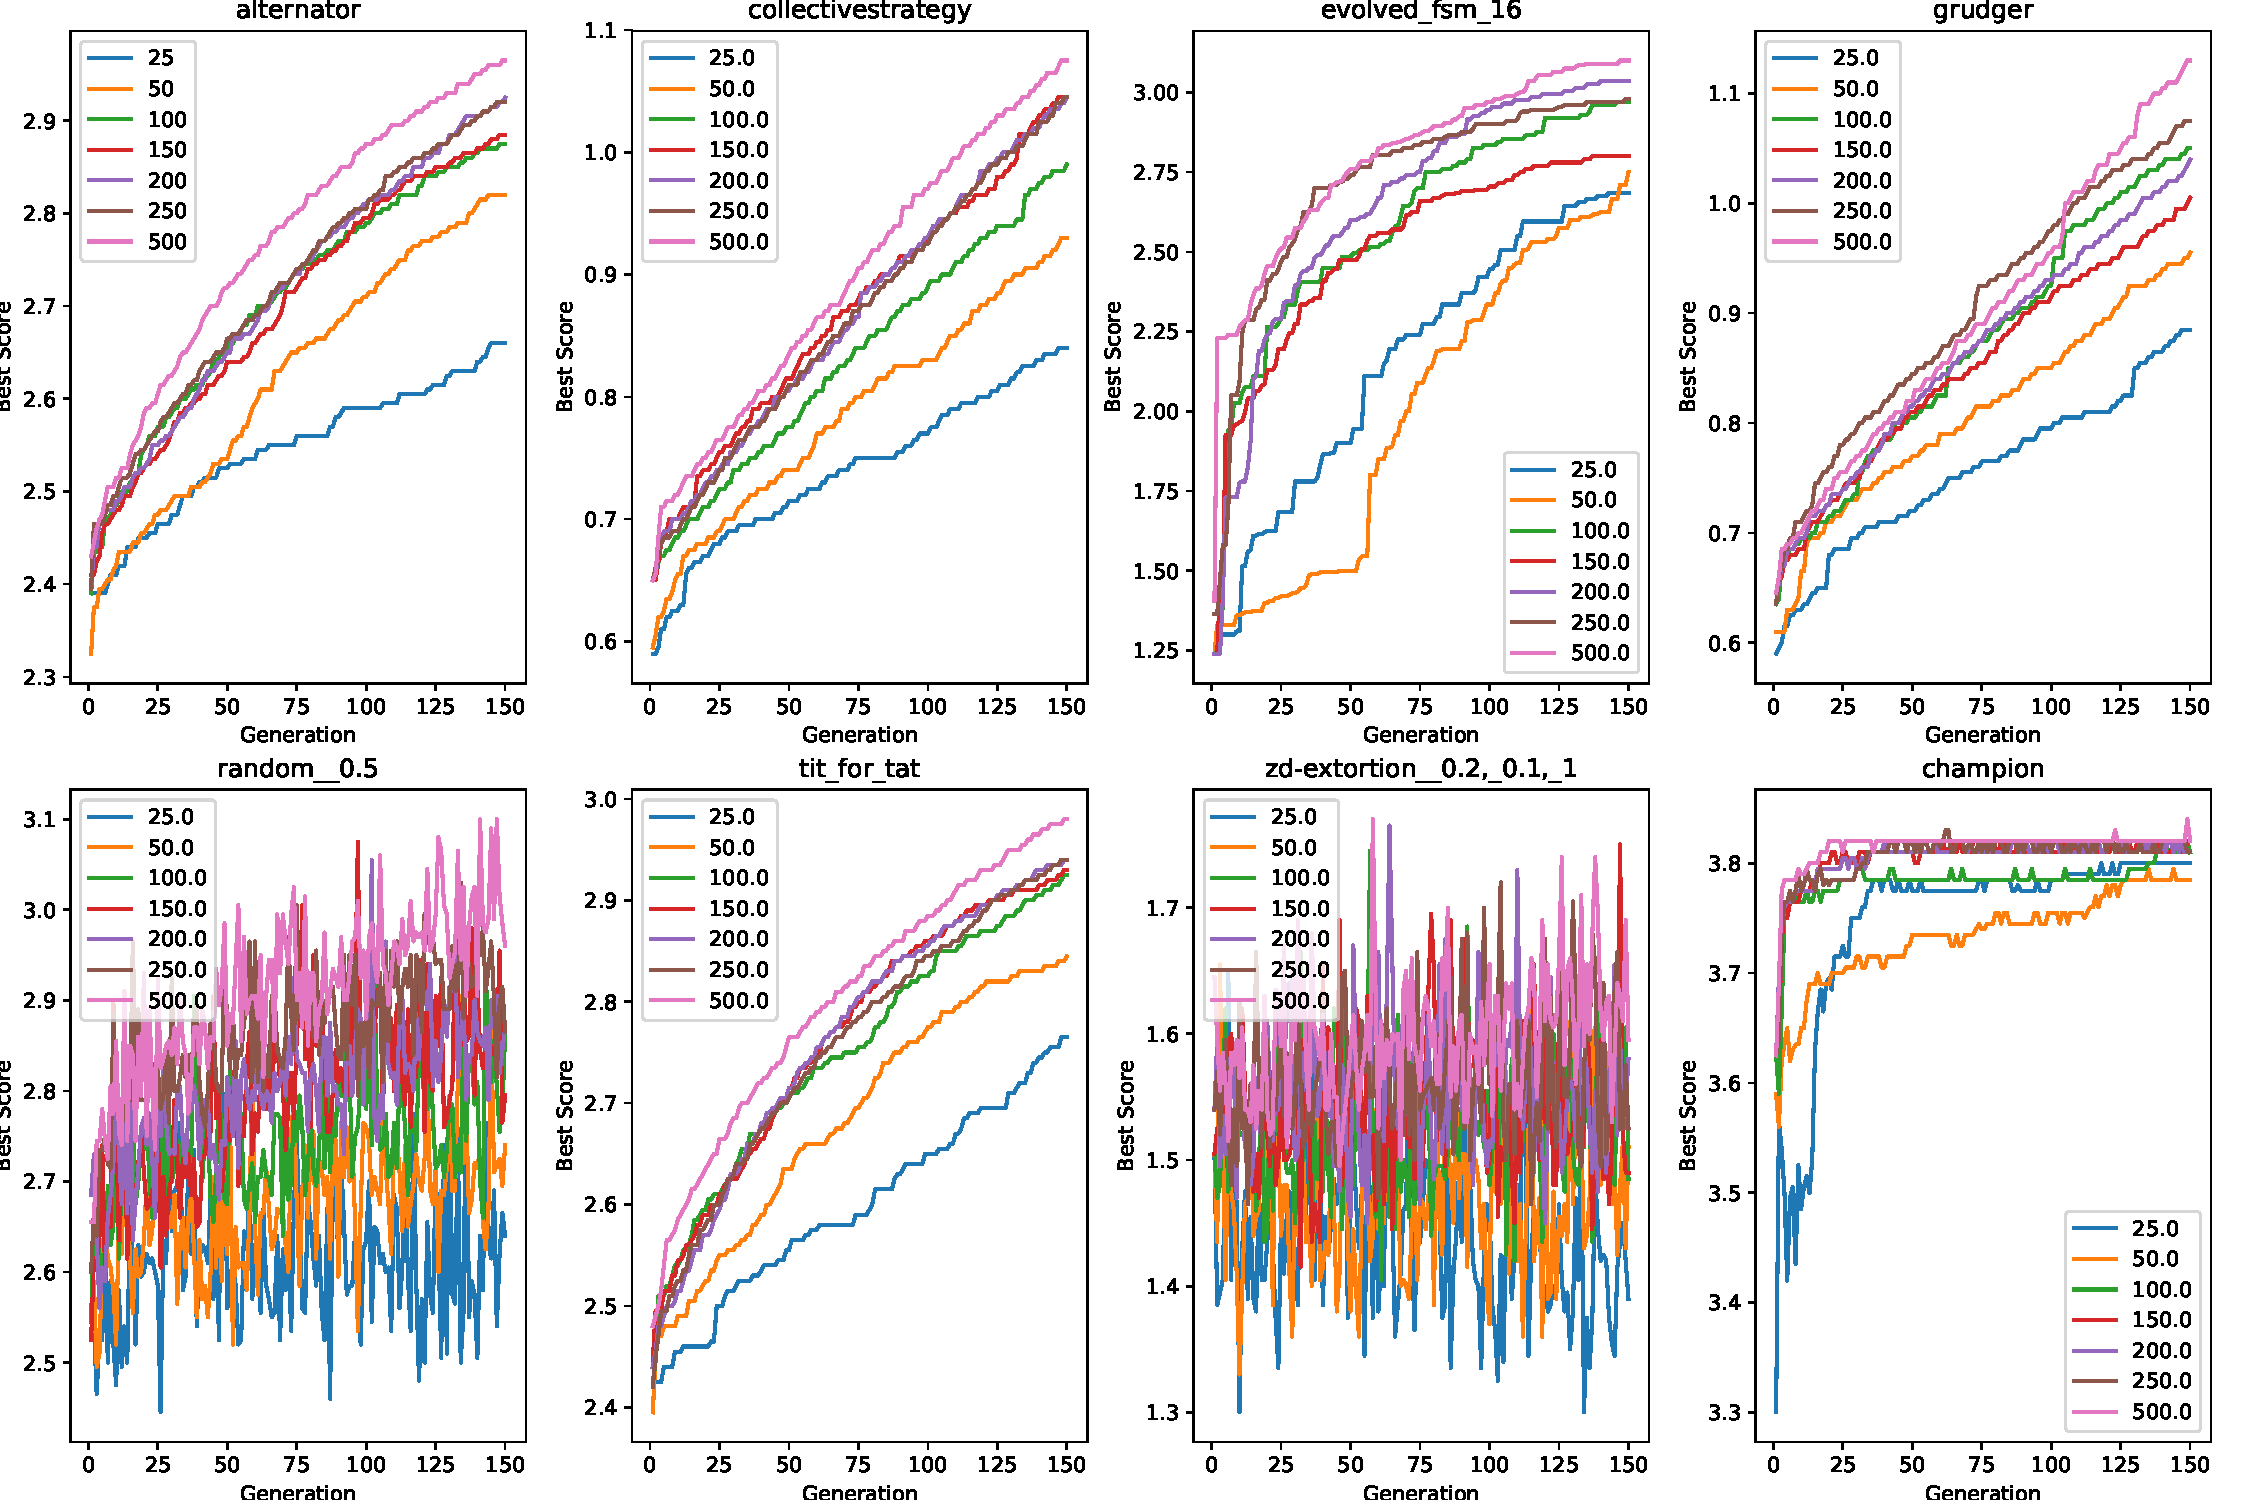
\includegraphics[width=0.8\textwidth, keepaspectratio, center]{./img/plots/INIT_POP_bs_v_gens_all.pdf}
    \caption{\textbf{Initial Population Size Analysis:} Best score per turn vs generation for different initial population sizes}\label{fig:INIT-POP-bs-v-gens-all}
\end{figure}

The improvements from the effect of population increase are non-linear from observation of Figure~\ref{fig:INIT-POP-mean-bs-v-init-pop-all}.
This figure shows the change in mean best score across population in the final generation against the population size.
The change in final best score for a population of 50 compared with a population of 250 is large in comparison to the same relative increase from 250 to 500.
This may suggest there are more efficient approaches to improving our final best score after a certain initial population is reached.

\begin{figure}[h]
    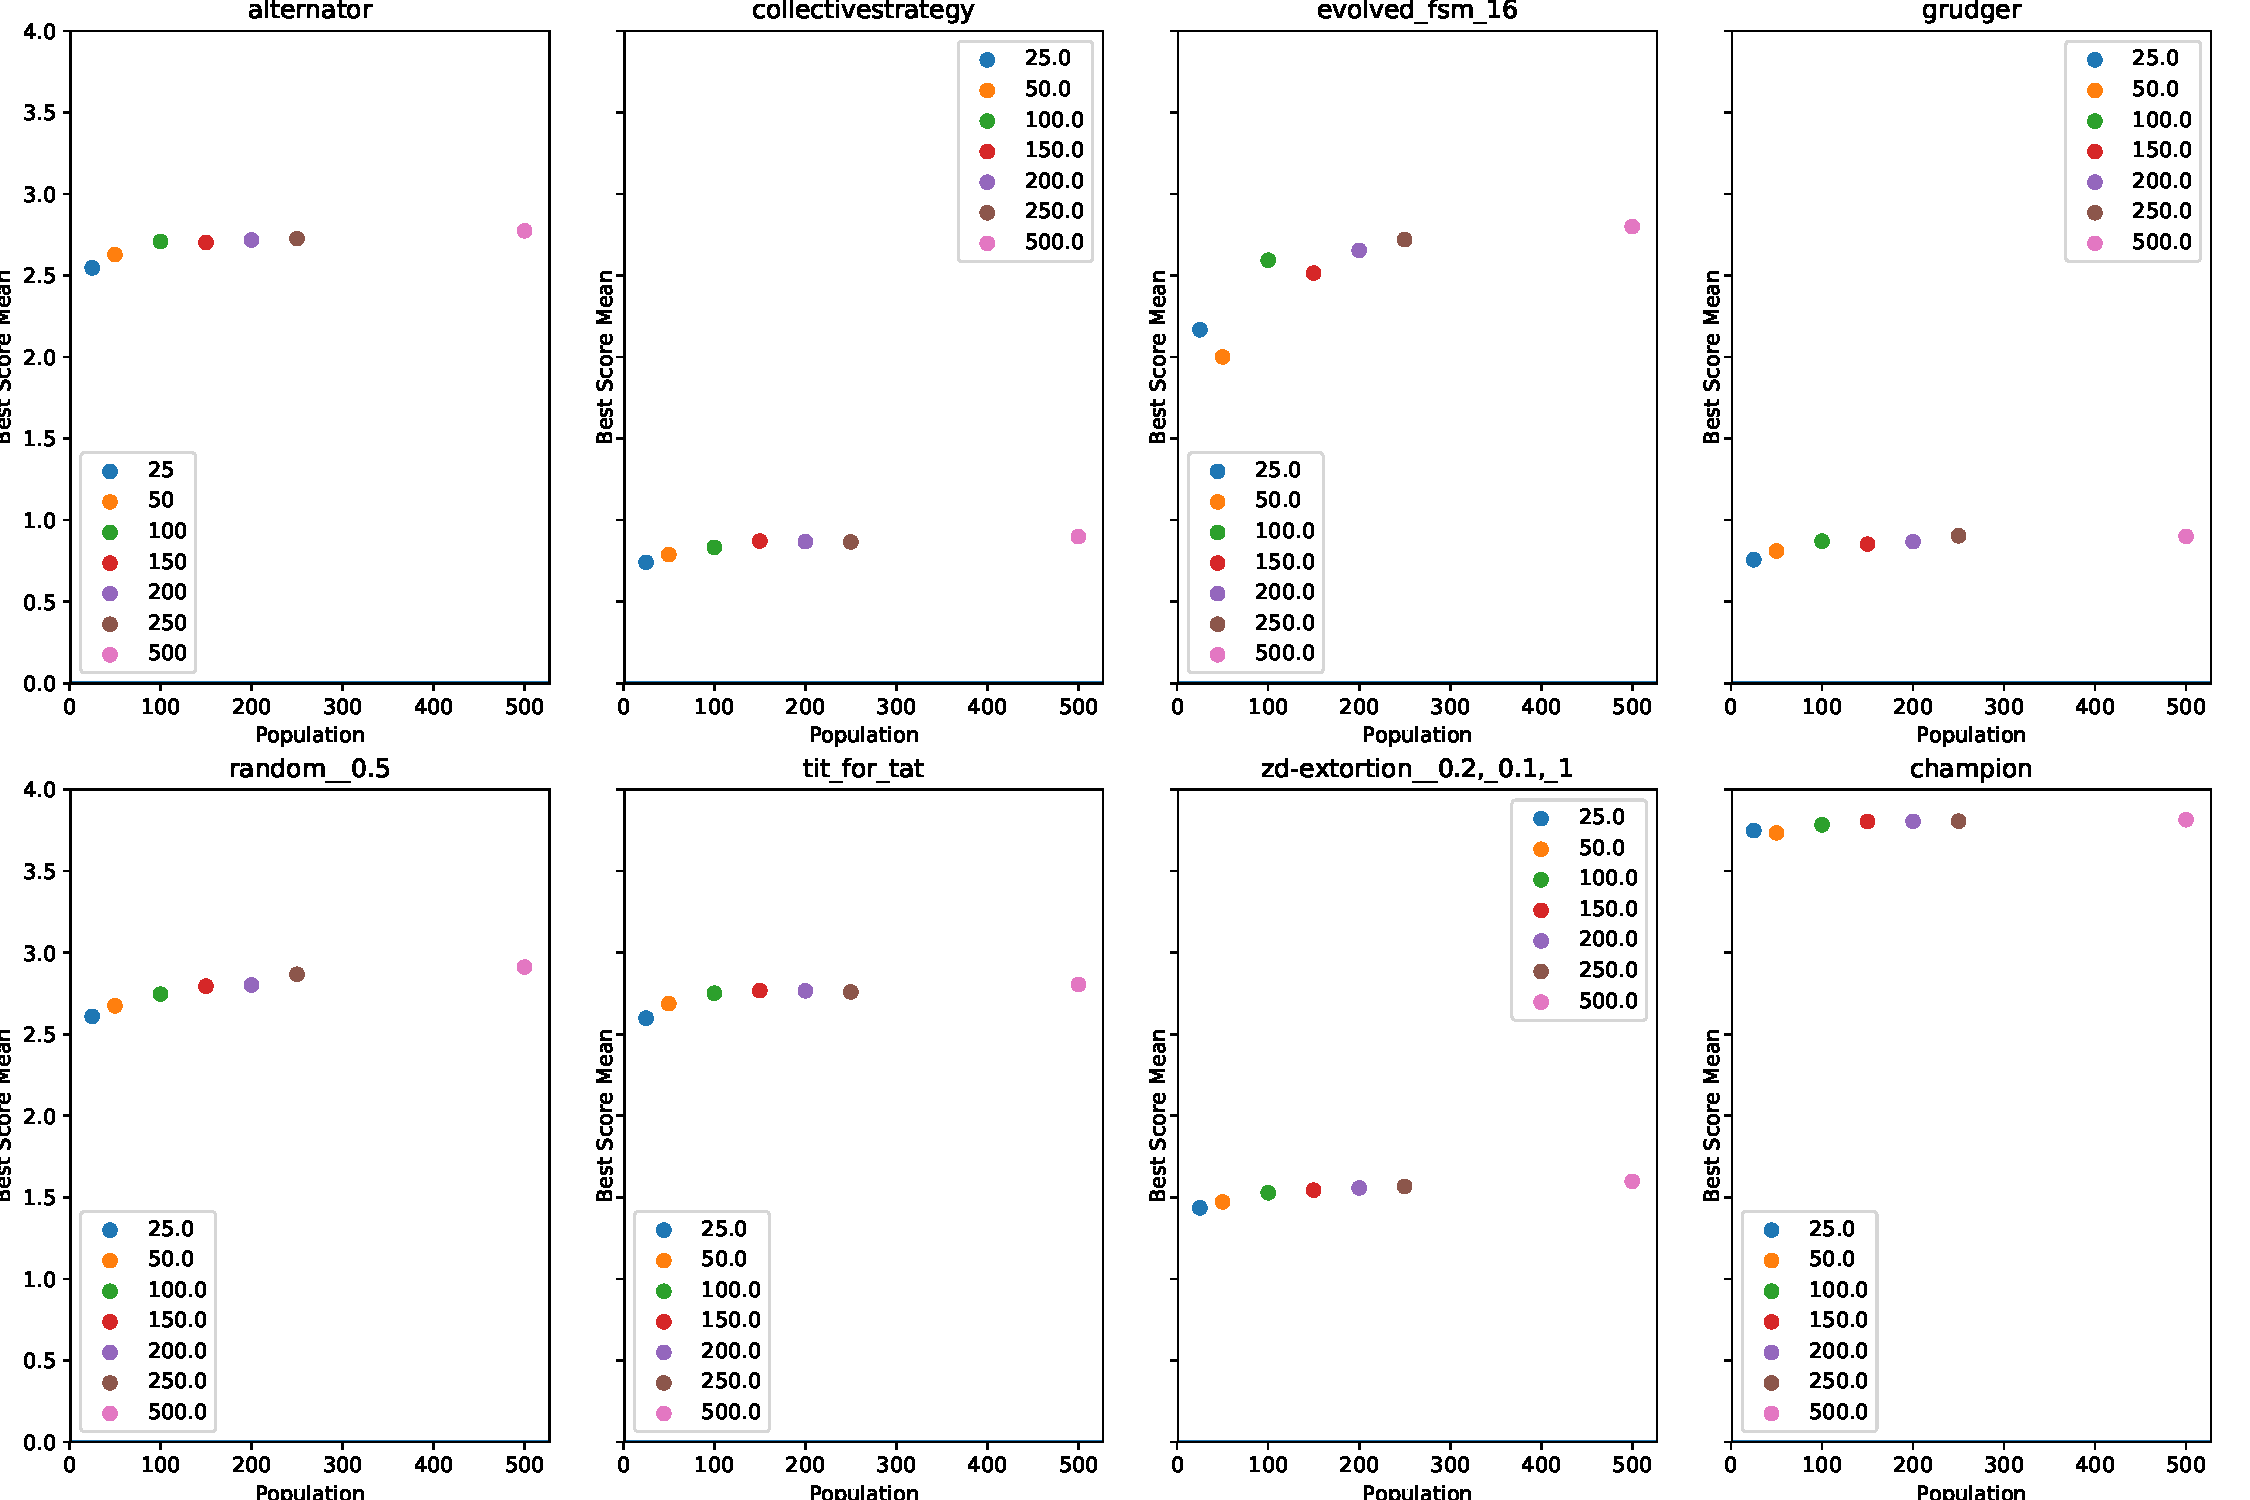
\includegraphics[width=0.8\textwidth, keepaspectratio, center]{./img/plots/INIT_POP_mean_bs_diff_v_init_pop_all.pdf}
    \caption{\textbf{Initial Population Size Analysis:} Scatter of mean best score vs different initial populations}\label{fig:INIT-POP-mean-bs-v-init-pop-all}
\end{figure}

None of these results have found a solution sequence (or at least we cant tell from the graph).
It is clear that larger initial populations do, on a relative scale, much better than small ones.
There are no large plateaus for the graph, so as we continue our research the initial population size will be increased to 150 to keep test computation times manageable.
The actual parameter we will use in the full analysis will be given consideration in Section~\ref{sec:conclusionOfApproach}.

\section{Generation Length Analysis}\label{sec:generationlengthanalysis}
Another major component parameter of a genetic algorithm is the number of generations it will run for before outputting a final set of members with solution sequences.
The number of generations has an influence on a number of different things within the algorithm:
\begin{itemize}
    \item {The total combinations of features that the algorithm can evaluate. 
    The more generations it runs for the more combinations of members we can evaluate a fitness for.}
    \item {The total number of low performers it removes in the population over the course of its run. 
    Each generation removes a proportion of its lowest fitness members.
    By definition of the algorithm we have a non-decreasing sequence of fitness scores; removing more lower fitness members will lead to a population of better or equal scoring members. }
\end{itemize}
Generation size differs from other parameters in the fact this is purely performance based, there is no changes to the inner mechanics of the algorithm only the amount of time it will run for.
A genetic algorithm with 1 generation is just a series of tests split into 2 results sets --- good performers and bad performers.
As we extend the number of generations we want be more focused on what happens to measured quantities normalised by generations, rather than any absolute improvement.

As a note on efficiency, the goal of finding the optimal solution sequence for each opponent would be solved by extending the generations to infinity, i.e exhaustively search the whole solution space.
This, however, is not a feasible solution, and so this section looks in to the effect of increasing generations has on improving a solution sequence with respect to the generations its run.
Here we will take generation lengths \(G \in [50,150,250,350,450,500]\) during these tests and a population size of 150.
The code in Appendix Snippet~\ref{apcode:generationChecker.py} shows how the approach the generation analysis was undertaken.

Figure~\ref{fig:GENS-mean-bs-diff-v-gens-all} shows how the mean best score across the population changes generation to generation normalized by generation.
It shows that over 150 generations the best scores against Alternator across its population increased, on average, by 0.0035 per generation.
From this we can observe how the number of generations has a declining effect the overall change in our mean best score per generation.
This trend is to be expected, when we are close to a maximum it is more difficult to randomly select which element in the sequence needs changing to improve a members score.
On this result we can conclude as we increase generations there is less and less benefit per generation.

\begin{figure}[h]
    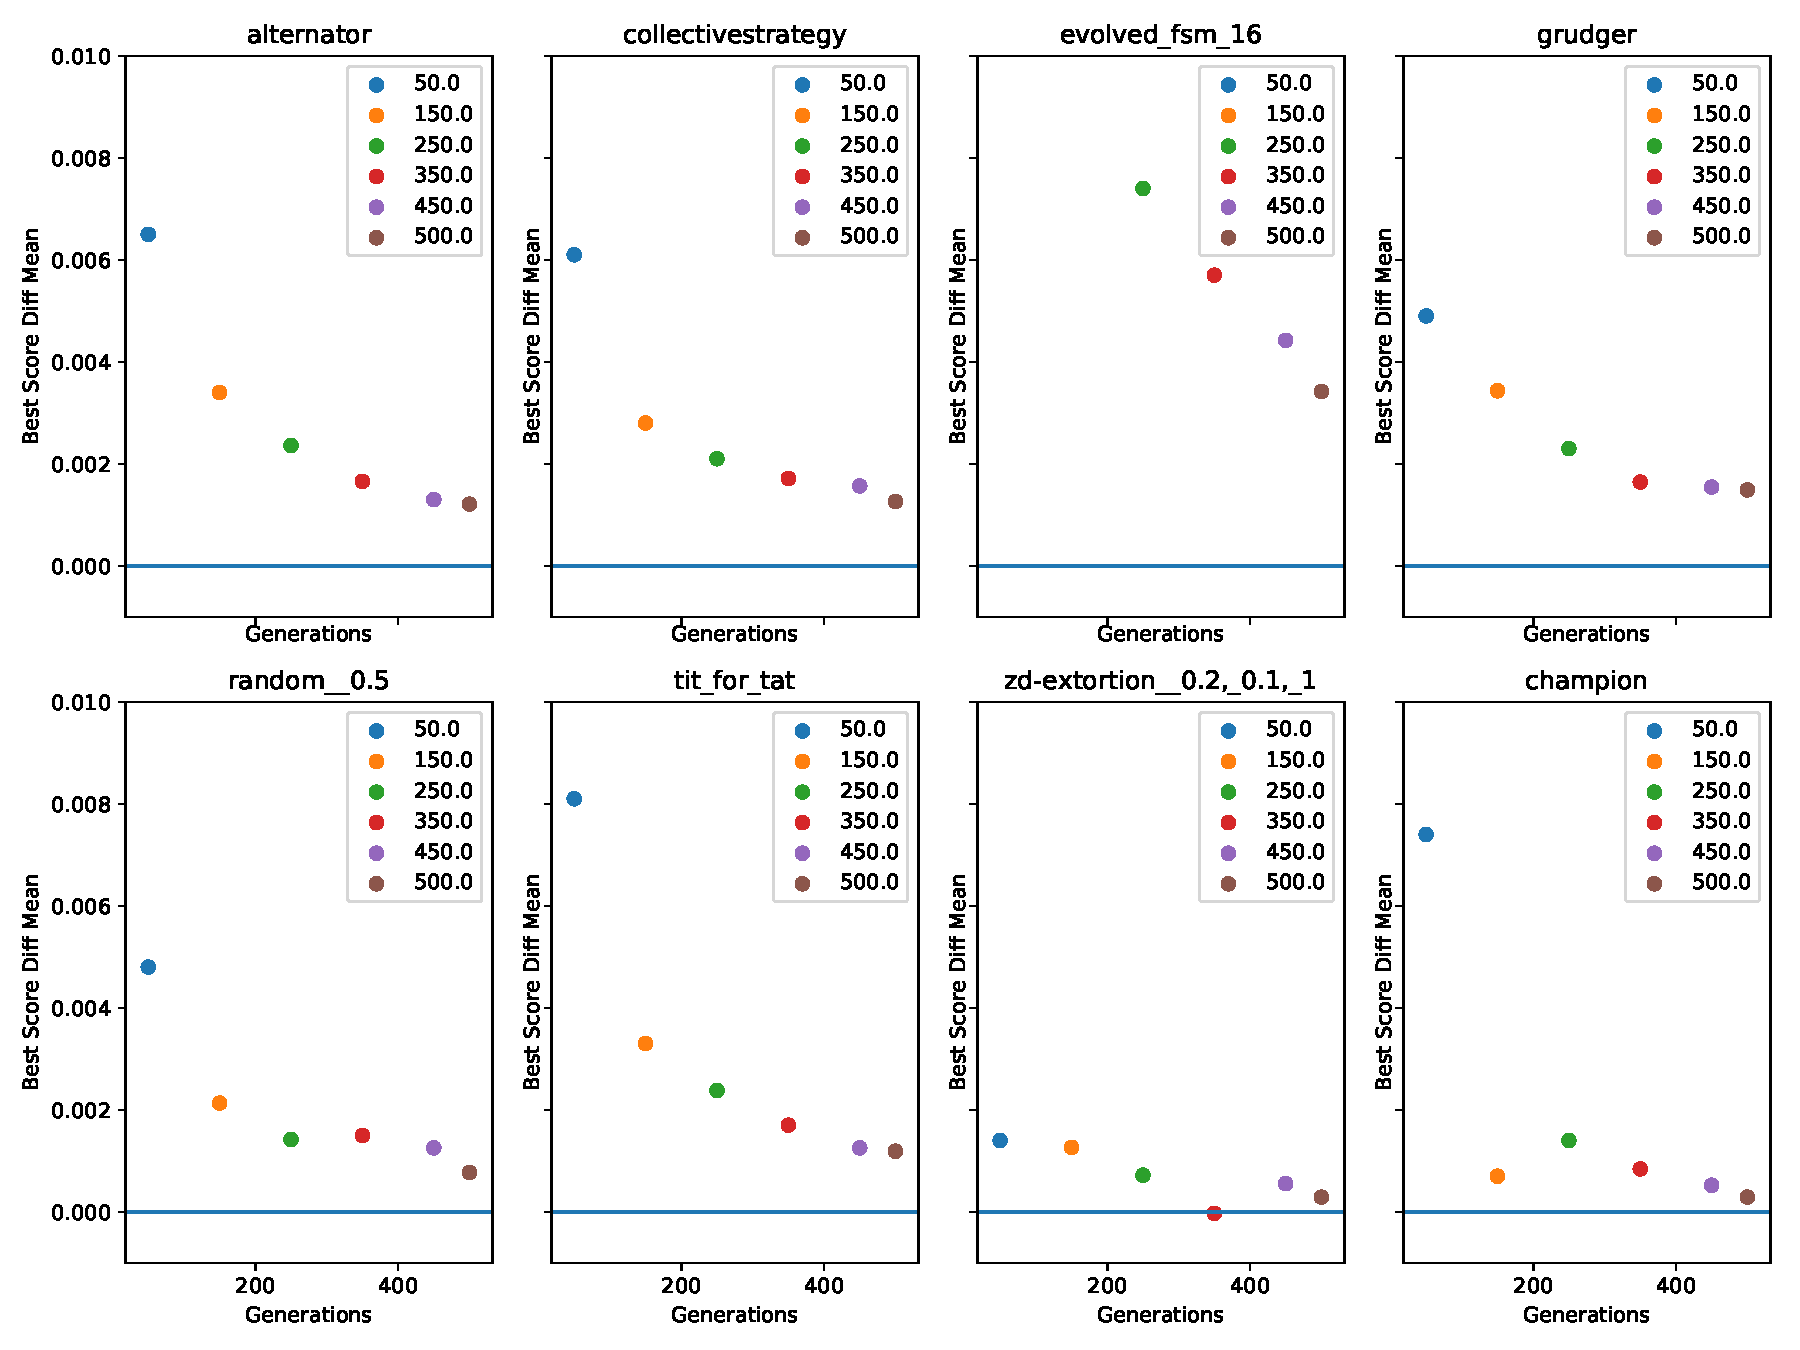
\includegraphics[width=0.8\textwidth, keepaspectratio, center]{./img/plots/GENS_mean_bs_diff_v_gens_all.pdf}
    \caption{\textbf{Generation Analysis:} Mean Best Score diff vs total generation lengths}\label{fig:GENS-mean-bs-diff-v-gens-all}
\end{figure}

Figure~\ref{fig:GENS-max-bs-v-gens-all} shows the maximum best score in a population once the analysis has concluded.
For most of the opponents 250 generations seems reasonable to reach a solution sequence as shown in the Alternator and Tit For Tat.
However, there are clear signs of local maximums occurring in the EvolvedFSM16 example.
In Figure~\ref{fig:GENS-max-bs-v-gens-all} EvolvedFSM16 has reached a better sequence in 150 generations than 500\footnote{These are independent trials and have different sequences.}, meaning that increasing the generation length doesn't necessarily mean finding a global maximum.
The complexities with local maximums during the generations lie with mutation rates and crossovers.
We will cover this in Section~\ref{sec:mitigatingLocalMaximums}

\begin{figure}[h] 
    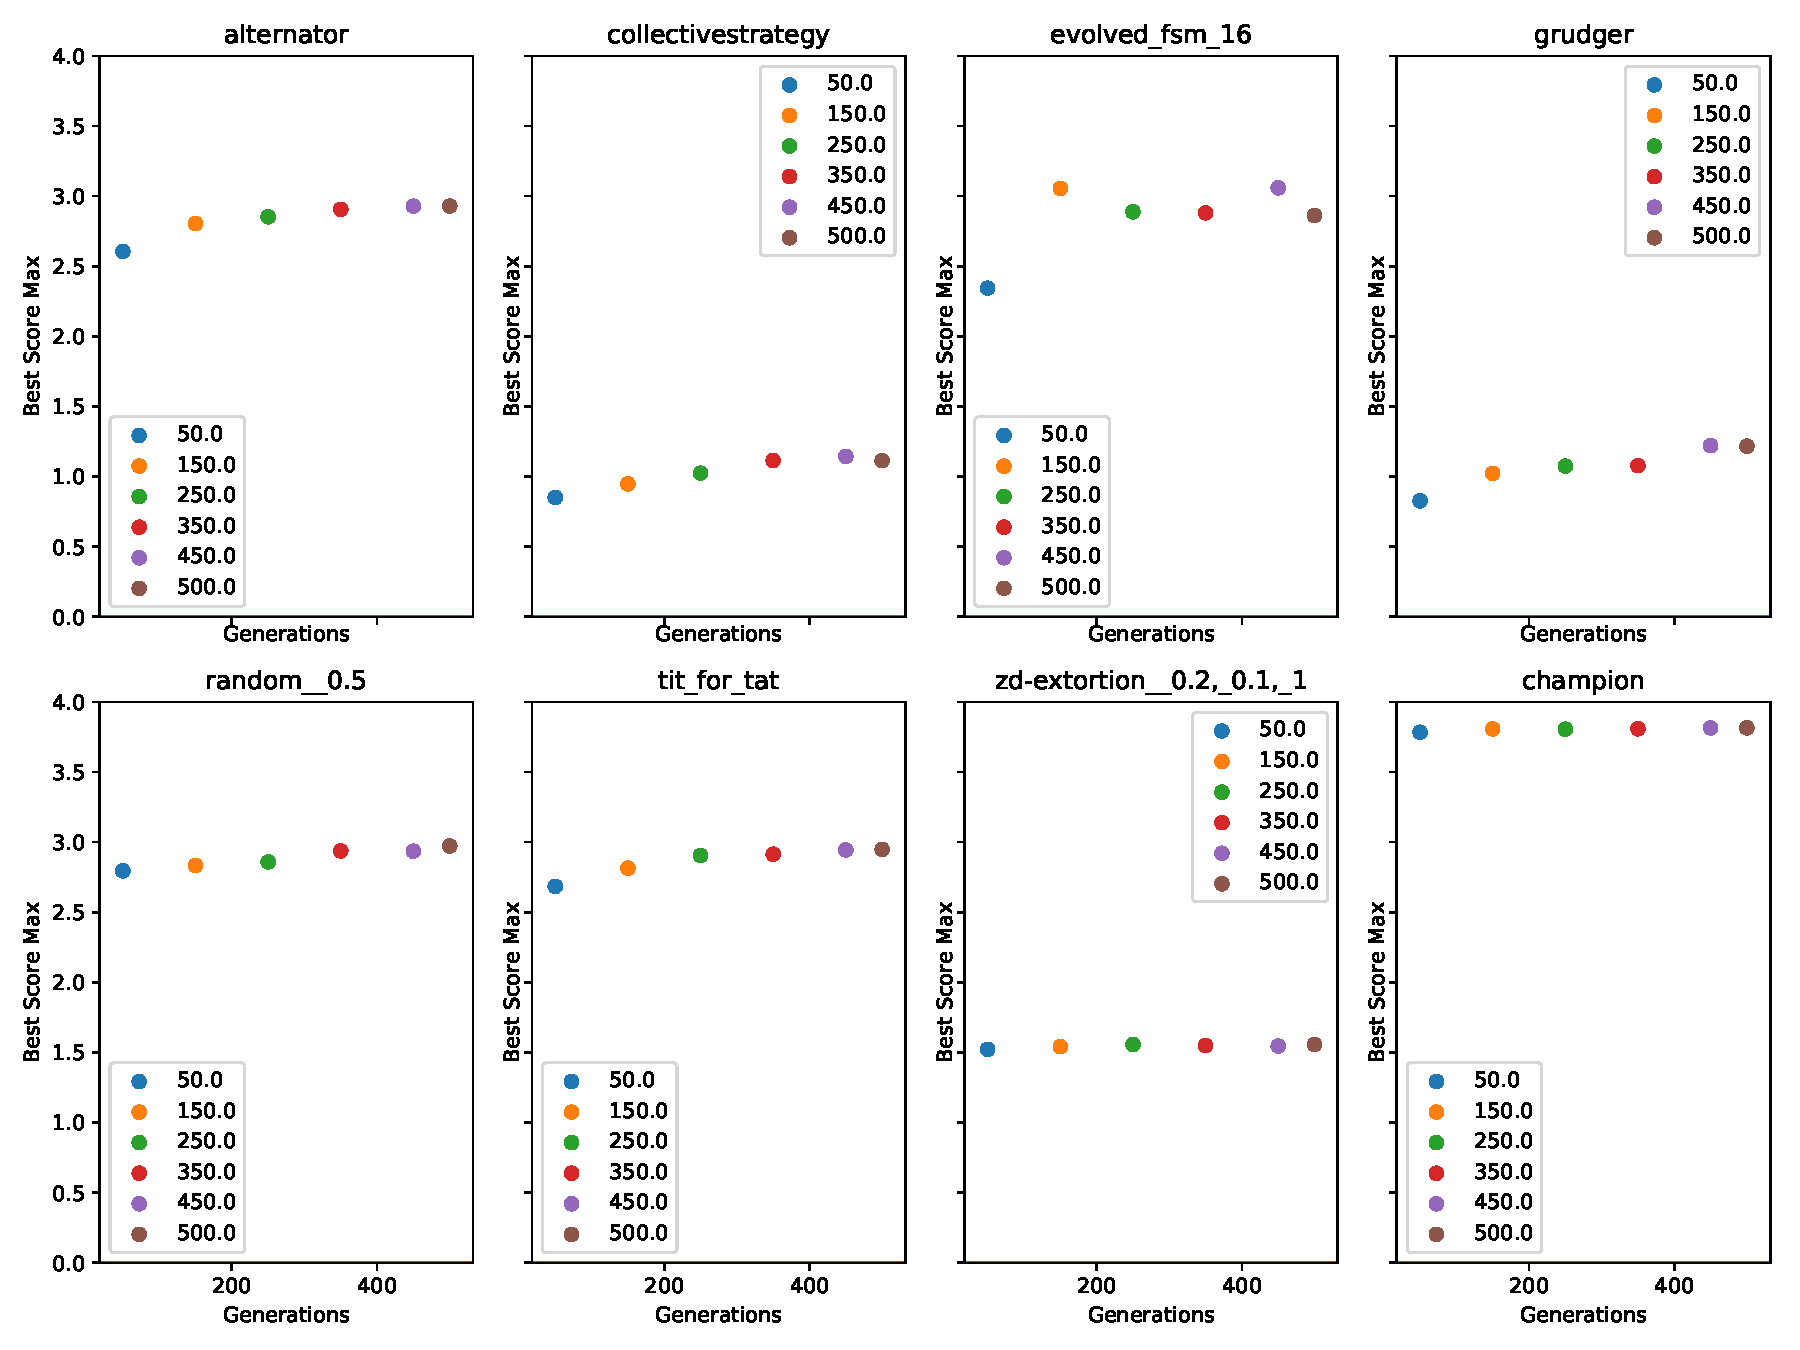
\includegraphics[width=0.8\textwidth, keepaspectratio, center]{./img/plots/GENS_max_bs_v_gens_all.pdf}
\caption{\textbf{Generation Analysis:} Max best score vs total number of generations}\label{fig:GENS-max-bs-v-gens-all}
\end{figure}

It is clear that a higher number of generations is preferred to find a better solution sequence.
As the number of generations increase each generation provides less of an improvement to the best scores.
This is due to the probability of finding a better solution sequence decreasing as we continue to improve a population.
The benefits of extending the generations are incredibly useful and due to the amount of computation time we can probably incorporate a high number of generations. 
However we may have better performance by altering another parameter of the algorithm.
The actual parameter we will use in the full analysis will be given consideration in Section~\ref{sec:conclusionOfApproach}.

\section{Changing Mutation Rate}\label{sec:changeingmutationrate}
This section looks at changing the amount of mutations that occur in our population and the number elements within a sequence each mutation effects. 
The default settings are a mutation frequency, $M_f$, of 0.1, meaning for every 10 members of our population that continue into the next generation one of these has some elements in its sequence changed.
And a mutation potency, $M_p$, of 1, meaning that every sequence that is mutated only has 1 element altered.
\begin{itemize}
    \item Is it beneficial for more/less than 1 in 10 members to be mutated generation to generation? (higher frequent mutation)
    \item Is changing one or more actions of a members' sequence the best way of mutating a member? (higher potent mutation)
\end{itemize}

These are two separate questions; first we will look at increasing the potency of our mutation.
Once we have found some information on how this effects our solution, we can look into the frequency of our mutations with the new potency as a permanent setting.

As a not on efficiency, this approach allows for an \(O(1)\) factor of computation scaling.
Changes in mutation are great candidates for an approach to reduce the number of generations to a solution sequence compared with other approaches.

\subsection{Changing Mutation Potency}\label{subsec:changingMutationPotency}
Changing the potency of the algorithm will provide small changes in a members features generation to generation.
Increasing the potency also has the effect of increasing the Hamming distance\footnote{Hamming distance: \(d(s_1,s_2)\) = the number of differing positions between 2 sequences \(s_1\) and \(s_2\).
For example: \(d(111,110) = d(CCC,CCD) = 1 \). This is covered in details in section~\ref{sec:distance_matracies}} between original and the mutated sequence.
 
Increasing potency too much has the potential for an algorithm that is too unstable for convergence. 
We can imagine a sequence as a vector in 200 dimensional space then a mutation for the \(i^{th}\) sequence element is the same as changing the vector in its \(i^{th}\) dimension.
Shortening this example to a vector in 3 dimensions (or a sequence of length 3) then a mutation is much more easily visualised.
Mutation potency should be kept low to keep consecutively mutated sequences more similar, keeping results of the mutation within a small neighbourhood of the original.
We will look into having mutation potencies \(M_p \in [1,2,3,5,10,15,20]\).

Figure~\ref{fig:MUT-POT-bs-v-gen-all} shows the best score as the algorithm progresses through generations.
There no clear benefit from increasing the mutation potency.
For example, in the Collective Strategy plot, having 15 genes changed per mutation still does not improve our score as much as changing only 2 or 3.
This may be down to chance of the random parameters used, however looking at more opponents than just Collective Strategy (EvolvedFSM16 for example) we find there is no clear benefit to increasing the mutation potency with respect to the overall best score against an opponent.

\begin{figure}[h]
    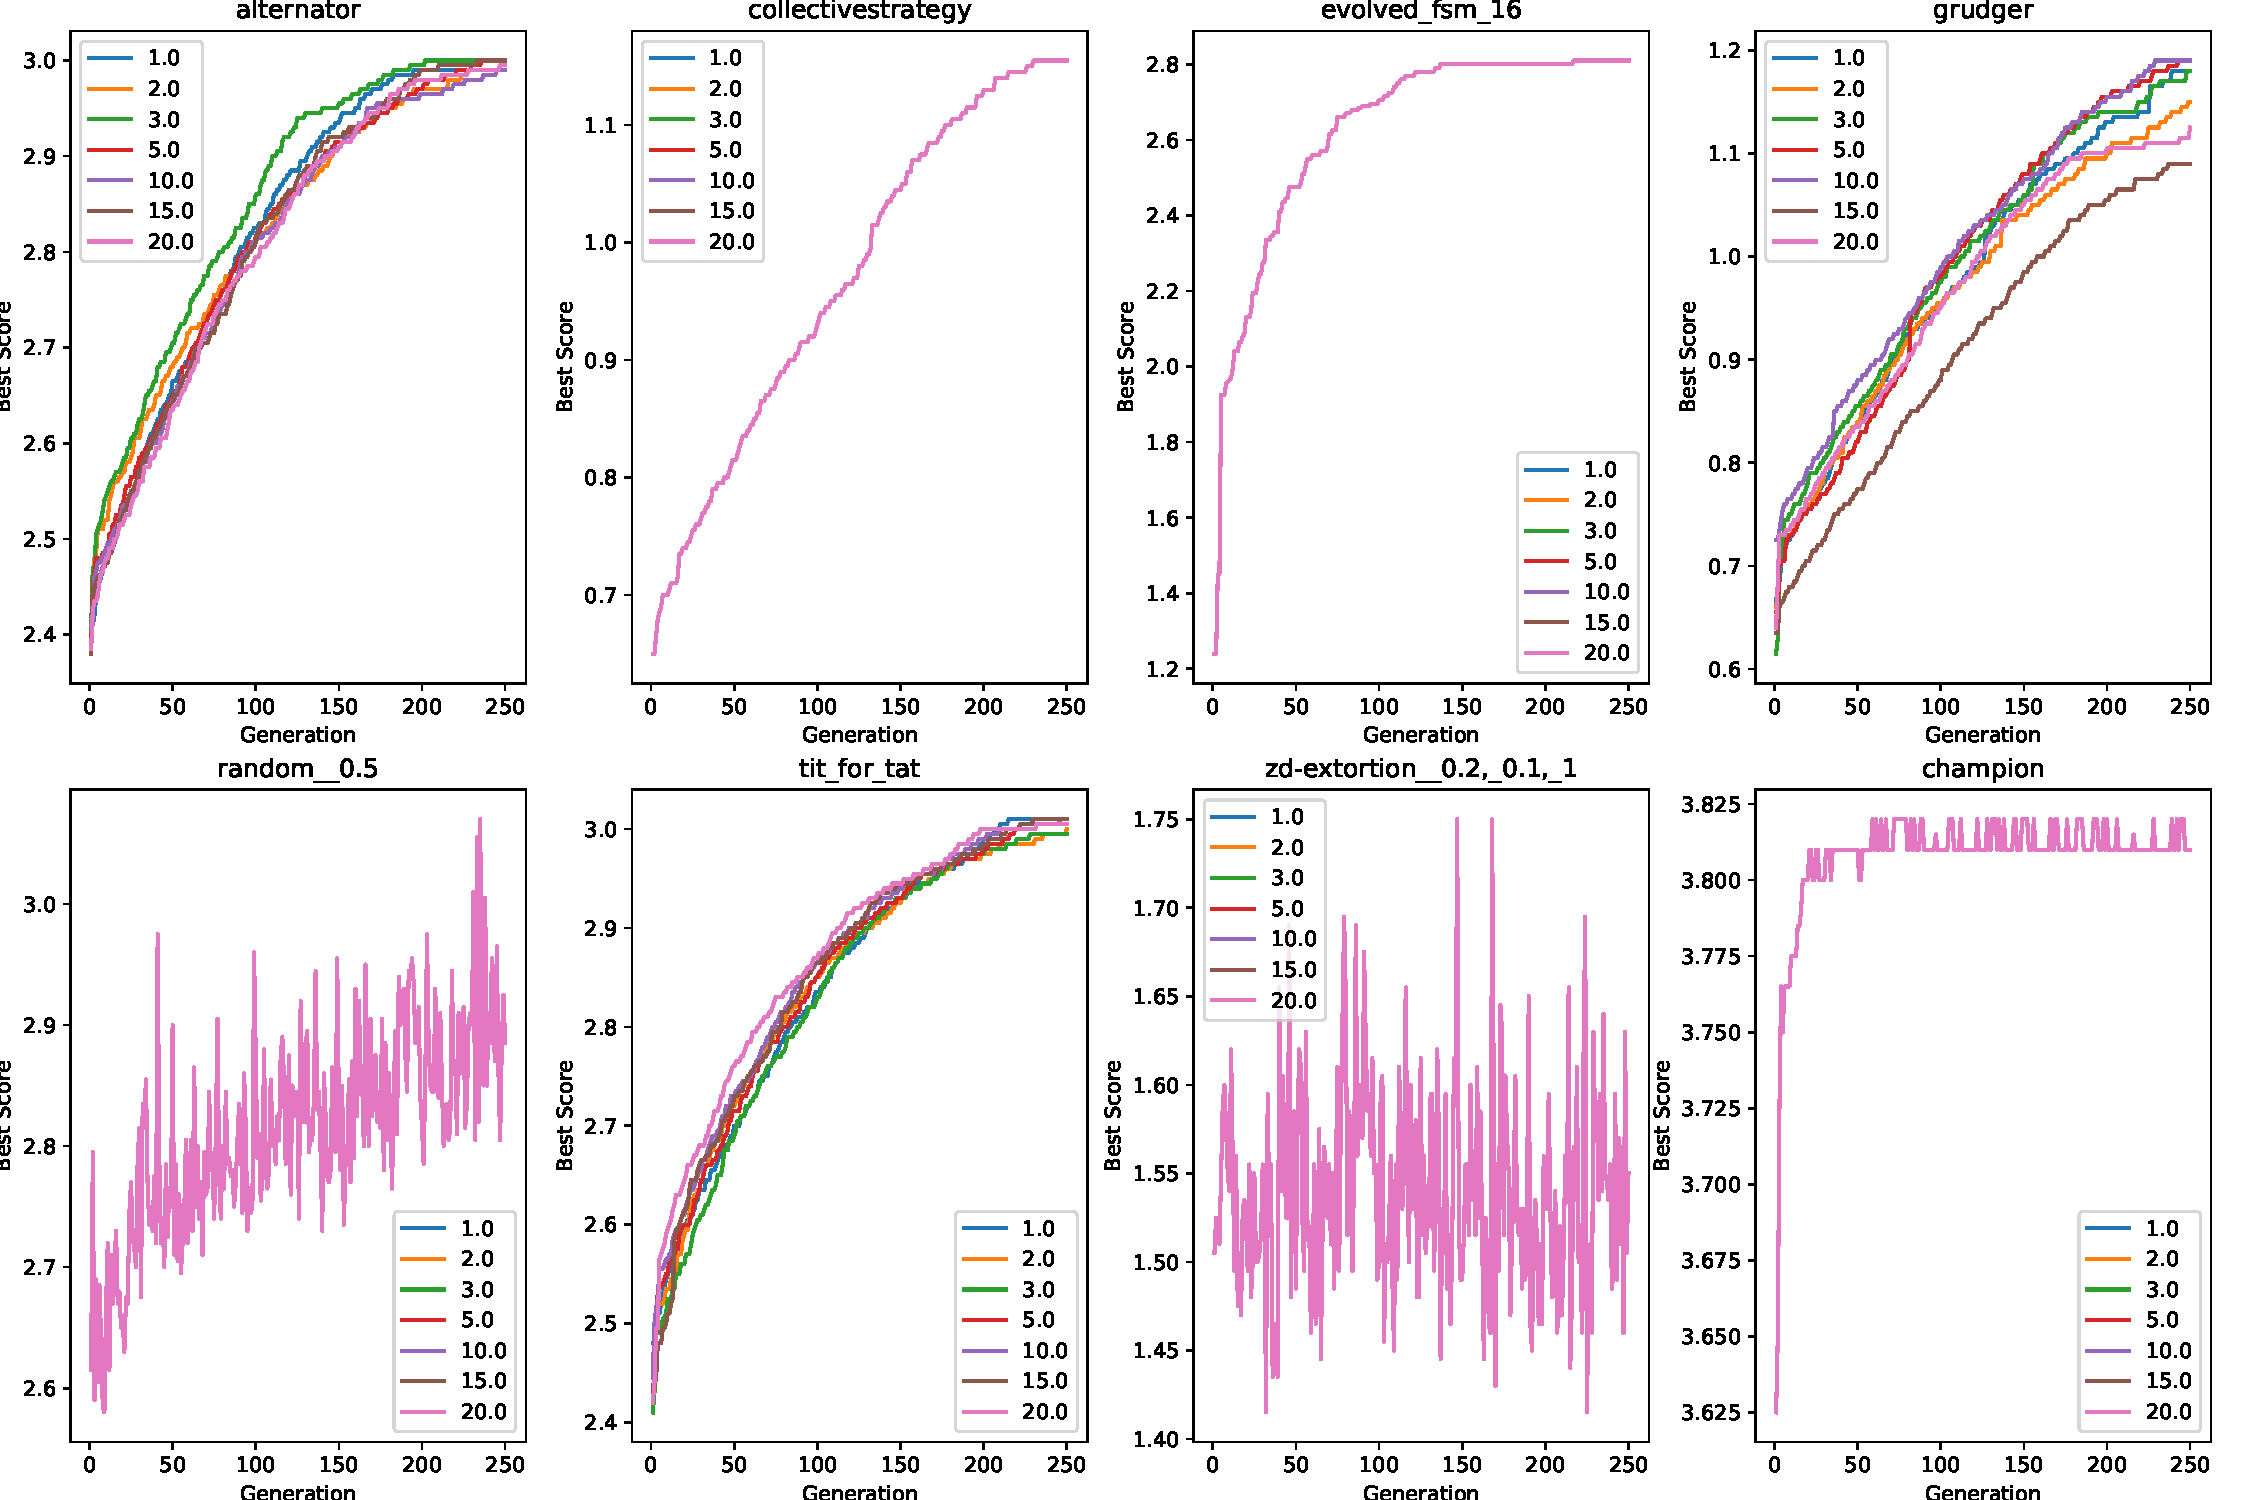
\includegraphics[width=0.8\textwidth, keepaspectratio, center]{./img/plots/MUT_POT_bs_v_gen_all.pdf}
    \caption{\textbf{Mutation Potency Analysis:} Best score vs generation for different mutation potencies}\label{fig:MUT-POT-bs-v-gen-all}
\end{figure}

Figure~\ref{fig:MUT-POT-bs-diff-v-pot-all} shows the trend of average increase of final best score across the population per generation against the mutation potency.
The increase in mean best score difference is not substantial and is most likely be down to chance in the areas it does change.
We see there is no sign these variables are correlated and hence can assume this parameter has negligible effect on the outcome of our sequence.
The actual parameter we will use in the full analysis will be given consideration in Section~\ref{sec:conclusionOfApproach}.

\begin{figure}[h]
    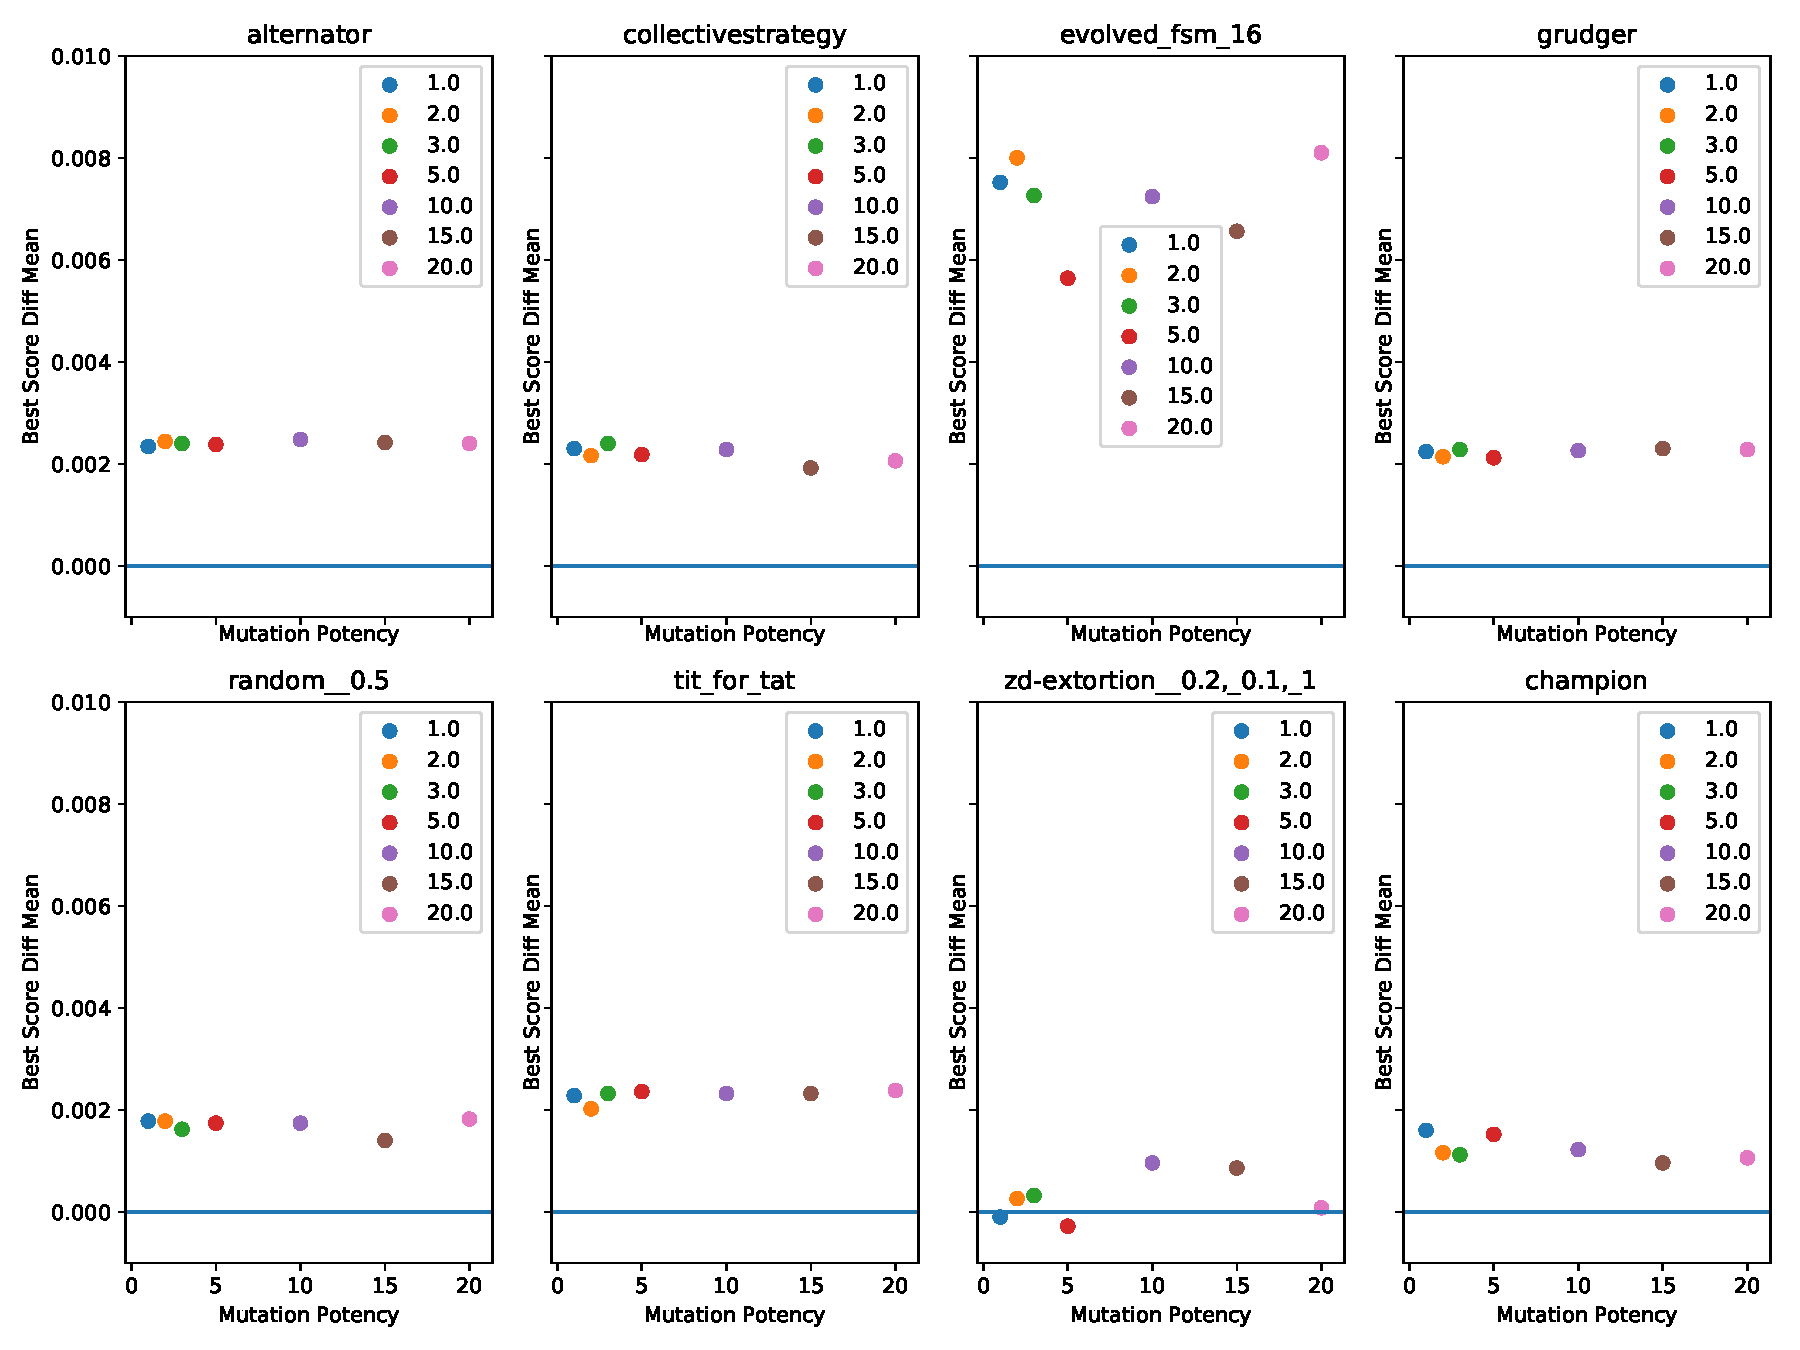
\includegraphics[width=0.8\textwidth, keepaspectratio, center]{./img/plots/MUT_POT_bs_diff_v_pot_all.pdf}
    \caption{\textbf{Mutation Potency Analysis:} Average best score diff vs mutation potencies}\label{fig:MUT-POT-bs-diff-v-pot-all}
\end{figure}

\subsection{Changing Mutation Frequency}\label{subsec:changingMutationFrequency}
In contrast to changing the mutation potency, increasing the frequency should allow us to generate more unique sequences generation to generation.
We will look at what happens when we run the genetic algorithm on a set of mutation frequencies \(M_f \in [0.1,0.2,0.3,0.4,0.5]\).
The code in Appendix Snippet~\ref{apcode:mutationFrequencyChecker.py} shows the code that completed this analysis.

Figure~\ref{fig:MUT-FREQ-bs-v-gen-all} shows how the best score improved generation to generation for each opponent across different mutation frequencies.
The results show there is little effect on the best score as we increase the mutation frequency.
However there is an interesting result that can be seen on the Grudger and EvolvedFSM16 plots; the algorithm has found 3-4 clearly different solution sequences each with different scores.
In the Grudger plot, we can see that the mutation frequencies of 0.15 and 0.2 produced higher scoring solutions than the other mutation frequencies.
In the EvolvedFSM16 Plot we have the same result.
There is no positive (or negative) correlation displayed in any of the opponents however.

\begin{figure}[h]
    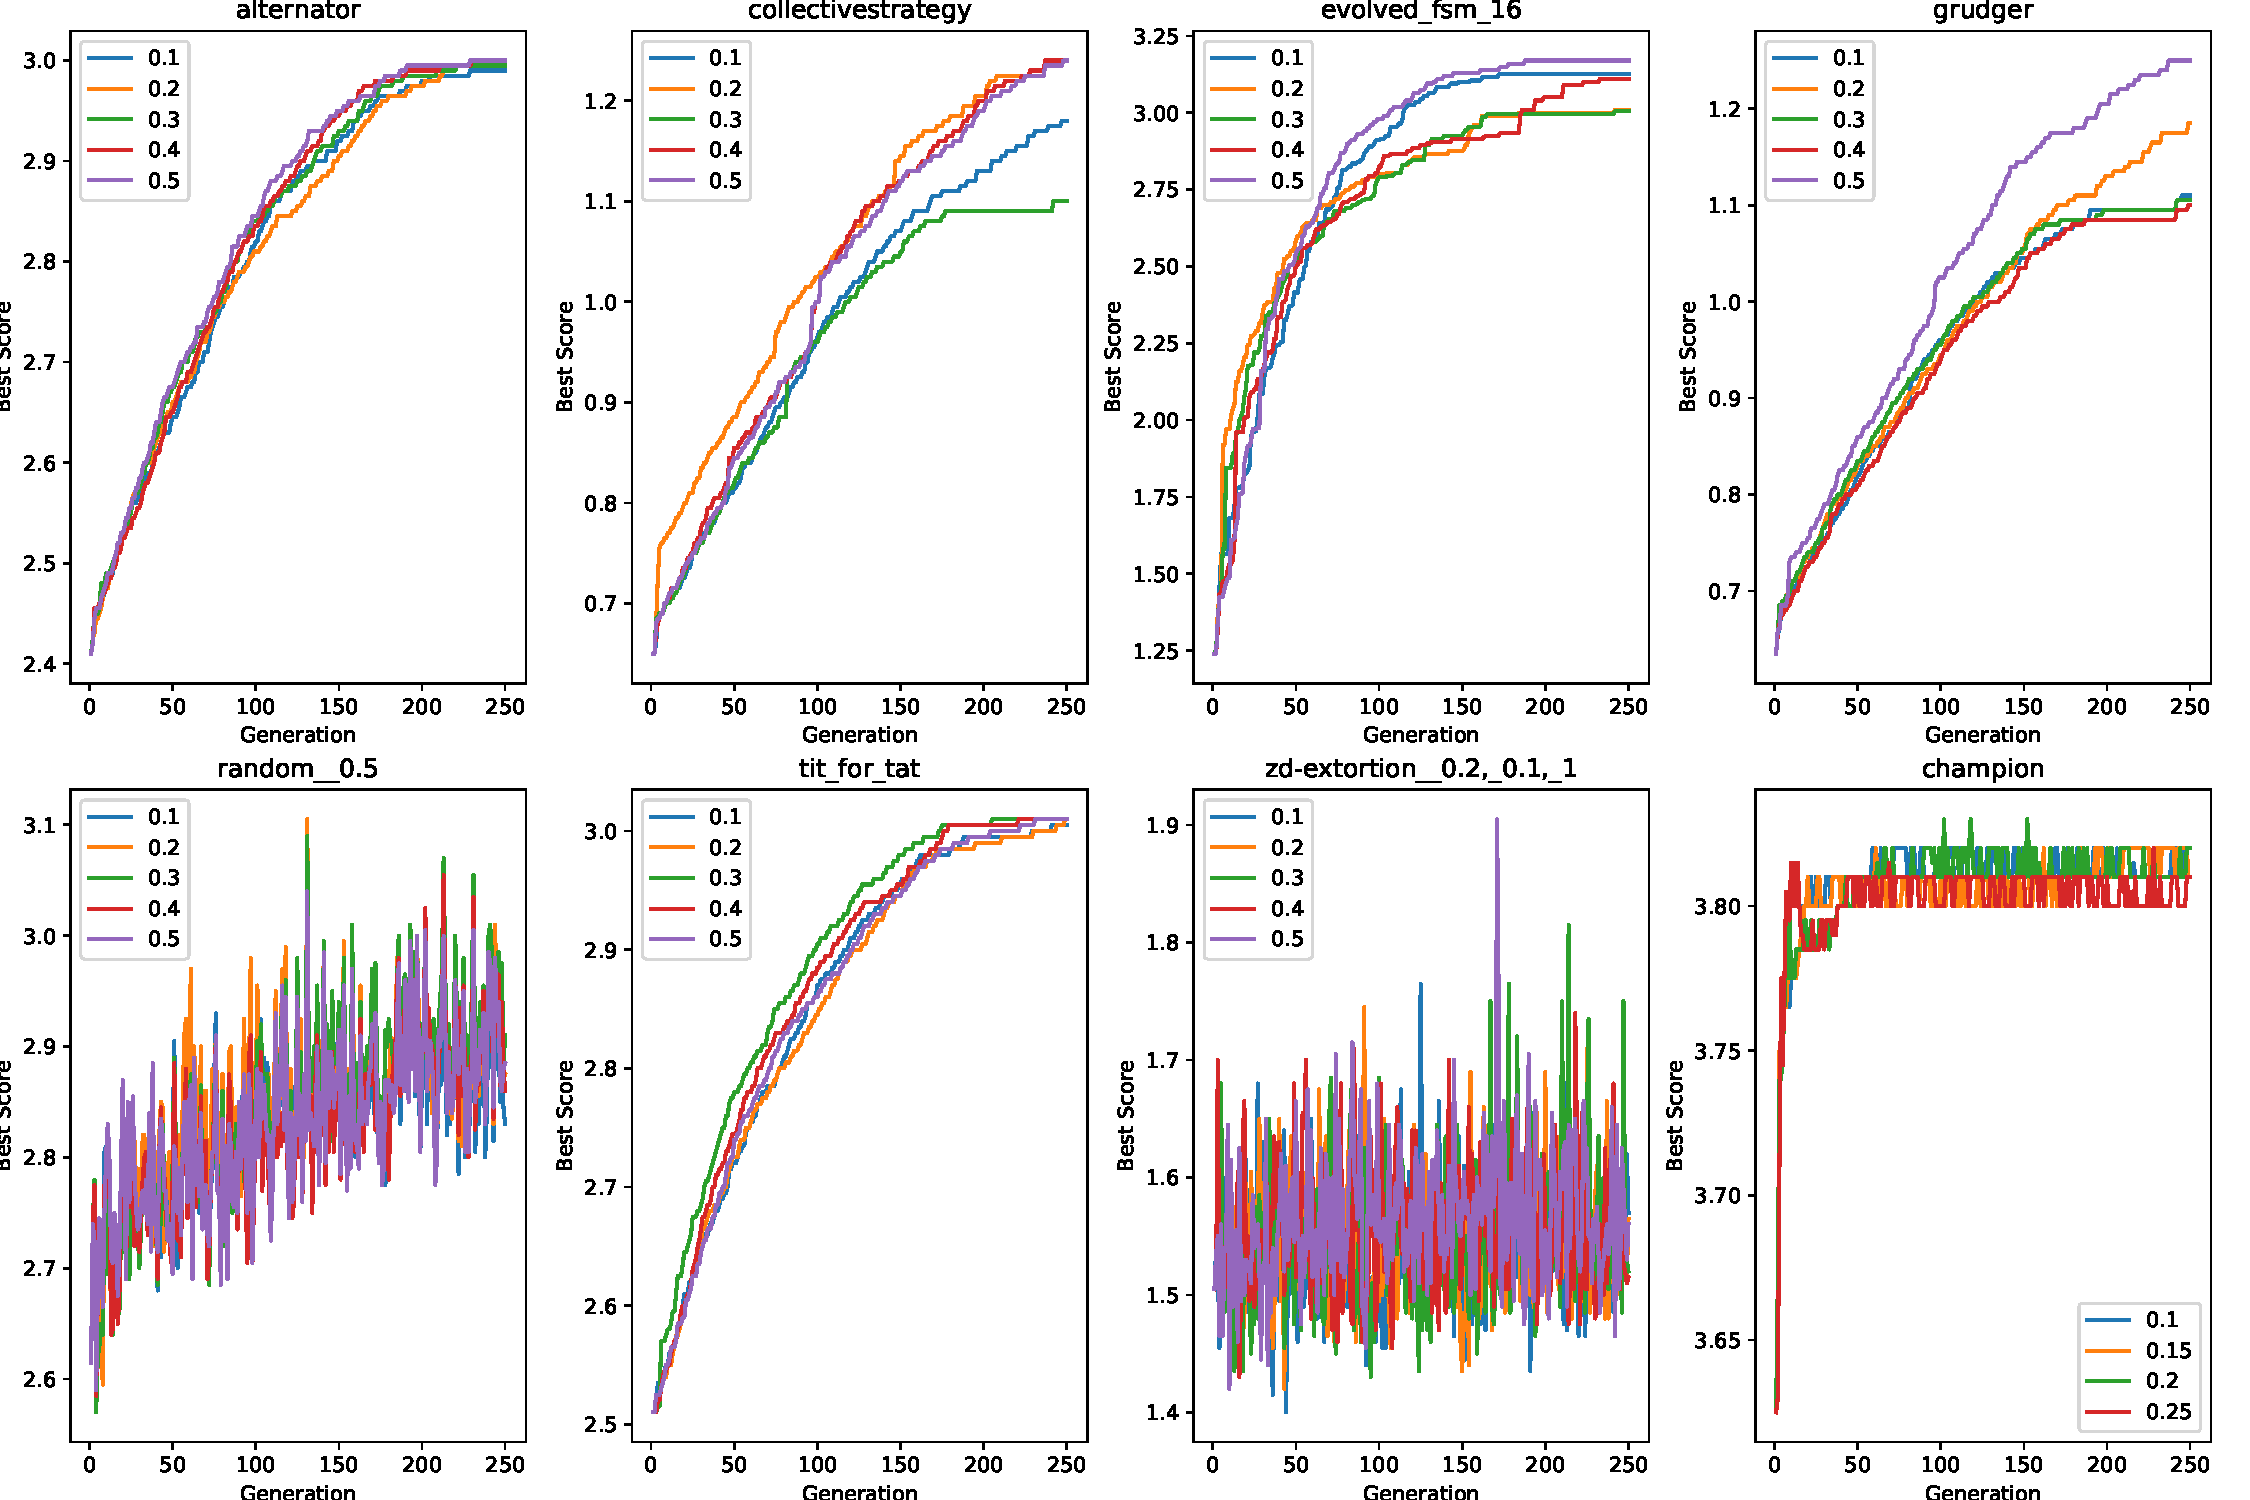
\includegraphics[width=0.8\textwidth, keepaspectratio, center]{./img/plots/MUT_FREQ_bs_v_gen_all.pdf}
    \caption{\textbf{Mutation Frequency Analysis:} Best score vs generation for different mutation frequencies}\label{fig:MUT-FREQ-bs-v-gen-all}
\end{figure}


% \begin{figure}[h]
%     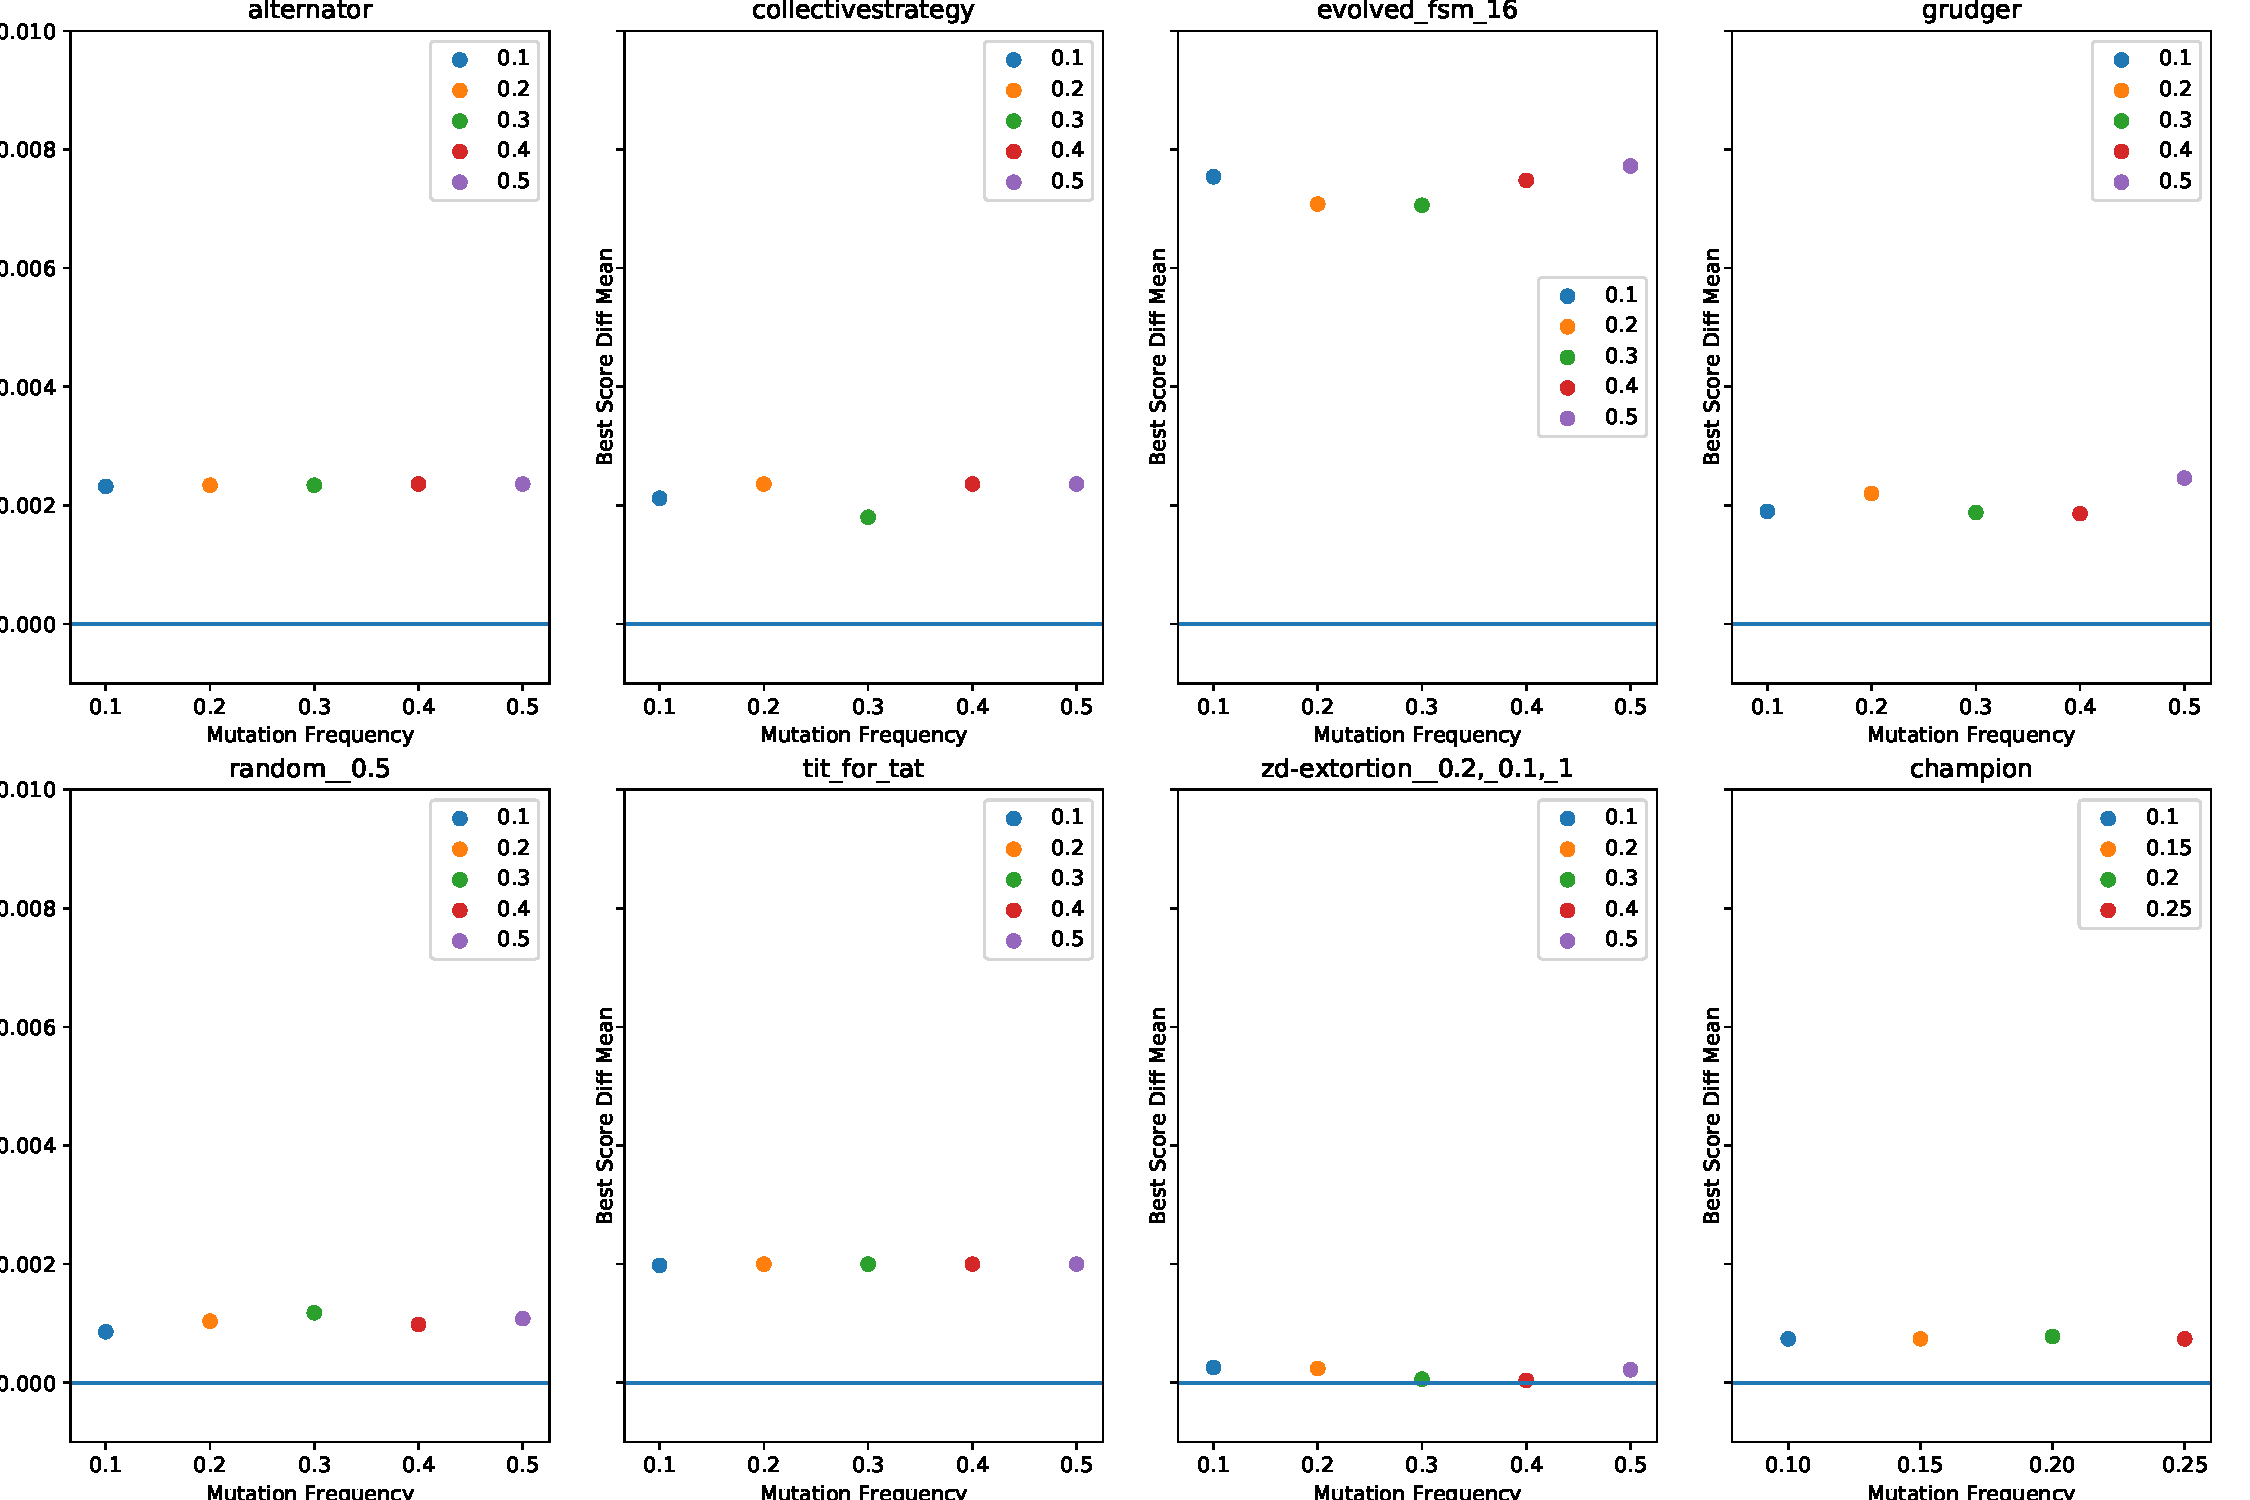
\includegraphics[width=0.8\textwidth, keepaspectratio, center]{./img/plots/MUT_FREQ_bs_diff_v_freq_all.pdf}
%     \caption{\textbf{Mutation Frequency Analysis:} Average best score diff vs mutation frequencies}\label{fig:MUT-FREQ-bs-diff-v-freq-all}
% \end{figure}

\subsection{Conclusions of altering Mutation parameters}
In the previous sections no improvements were found from altering any of the two parameters. 
The default of $M_f=0.1$ and $M_p=1$ will be used in further analysis, and the actual parameters we will use in the full analysis will be given consideration in Section~\ref{sec:conclusionOfApproach}.

These sections did show, in a clear manner, that there were local maxima found. 
Section~\ref{subsec:changingMutationFrequency} showed clearly that sub optimal solutions for EvolvedFSM16 and Grudger were common.
Section~\ref{sec:mitigatingLocalMaximums} will discuss approaches we can take to reduce the chances of this happening.

\section{Mitigating Local Maximum Solutions}\label{sec:mitigatingLocalMaximums}
Local maxima have clearly occurred when the algorithm calculates sequences for opponents Grudger and EvolvedFSM16.
There may be other occurrences we have not observed.
Each stochastic opponent is also incredibly difficult to understand whether a solution is actually found, this is discussed further ing Section~\ref{sec:stochasticOpponents}


Figure~\ref{fig:MUT-FREQ-bs-v-gen-all} shows that there are clearly multiple distinct score plateaus reached for the Grudger opponent.
The difference between Grudger and the other opponents considered is that the Grudger has a singularity where its behaviour changes.
The change in behaviour is not uncommon, Tit For Tat, Collective Strategy and others work in a similar way and in all cases the algorithm has managed to identify this behaviour and adapt to overcome its negative effects.

Grudger is an opponent which it is possible to attain a local maximum score and be `trapped' in this solution sequence.
If we look at a random start sequence and then the end sequence after 250 generations we can see that the genetic algorithm is learning defect after some point and cooperate before.
This is due to the fact a `good' solution will cooperate to the point of a defection and end in lots of defections after it has already defected counter Grudgers' harsh behaviour (see Section~\ref{sec:strategiesOfInterest} for the Grudger strategy).

%Grudger best start: \(C:[6,8,2,1,2,1,6,1,2,2,4,2,1,1,2,10,1,1,1,3,1,3,1,1,1,1,2,2,1,1,1,2,3,5,2,2,2,1,1,2,1,1,4,1,2,1,1,1,2,3,1,1,2,2,1,7,3,2,1,2,3,1,1,5,1,1,1,1,1,1,1,1,1,1,4,1,1,1,1,4,2,1,1,3,1,1,2,3,4,1,1,3,2,4,2,1,2,3]\)
Grudger best start: C$6,8,2,1,2,1,6,1,2,2,4,2,1,1,\ldots$ (No pattern is obvious.)

Grudger best end: C$22,178$

We may be able to identify a way to mitigate this singularity effect by looking at the difference between 2 opponents whose strategy differs by their forgiveness parameter.
Grudger and Tit For Tat differ in their strategies in two ways:
\begin{itemize}
    \begin{item}
        Grudger never changes its mind.
        There is one change in behaviour for the entire game, unlike Tit For Tat.
        The algorithm then only has a single opportunity to observe this per population per generation meaning the behaviour is much less frequently encountered.
    \end{item}
    \begin{item}
        Grudger will not forgive and becomes a `dumb' only defect opponent.
        This means that the move the algorithm picks up the effect of a single defection in its sequence it starts playing a `dumb' opponent.
        A random start of Cs and Ds puts the likelihood of at least 1 defection occurring in the first 10 moves at above \(99.99\% \).
        This swap from `smart' to `dumb' will, most likely, always occur in the first 10 moves;
        the only way of extending the `smart' player is to add a cooperation to the end of the starting Cs.
    \end{item}
\end{itemize}

To investigate this we will play two totality games against grudger, one of all Cs and one of all Ds, shown in Snippet~\ref{code:gudgerTotalities}. 
These games show we should be converging on a totality of Cs rather than what its doing, finding the totality of Ds after a number of cooperations.
This is probably because the algorithm initially limits its best score per turn once the first generation is complete and a cut-off defection has been established for each of the initial population.
The crossover method between generations then doesn't provide enough of a mix up to allow the algorithm to escape the local minimum by switching a subsection with a sufficiently different, potentially better, subsection.
Then when it comes to mutating, there is little any number of mutations can do to drastically change large sections of the solution sequence without knowing exactly where to target.

\begin{figure}[h]
    \inputminted{python}{code_snippets/grudgerTotalities.py}
    \caption{Grudger matches against totalities}\label{code:gudgerTotalities}
\end{figure}

The example totalities, shown in Snippet~\ref{code:gudgerTotalities}, are edge cases and would be rarely encountered as a starting point in the random initial population.
Because of this, the algorithm has to shuffle towards the potential benefit of using these totalities rather than start with analysing them.
Our case against grudger requires the algorithm to attempt this shuffle towards a totality after encountering the grudging effect.
This would then require the algorithm to select the first defection move and change it to a cooperation move all by chance.
The likelihood of this occurring is incredibly small, and starting at common or uniform sequences would be more beneficial to searching to solution space, as posed in Section~\ref{sec:alteringinitialpopulation}.

\subsection{Ineffective Approaches of Altering Crossover And Mutation}\label{subsec:ineffectiveApproachOfAlteringCrossoverAndMutation}
The process of converging to Ds when building a solution against grudger then sheds light on the process the algorithm takes to find a solution.
If the algorithm is to find the optimal solution sequence, it must take a crossover and mutation path which doesn't cut off better paths as the algorithm work our way towards good solutions.
This is much easier said than put into practice due to the way the algorithm `cuts off paths'.
The current technique is taking halves from 2 members and merging them, potentially removing successful relationships between elements in both the first and second halves.
If we reverse this thinking and try to alter our crossover design and mutation rate such that, instead of `cutting off' a path by taking large sections of each member, it may be possible to `build' new ones using more, smaller, sections of the 2 parents.

We can re-design the crossover to switch up smaller subsections of the solution sequence then allow the mutations to optimise these sub-sequences.
The current design is shown in Figure~\ref{fig:oldCrossover}.
We want to allow the crossover to have more of an impact on optimizing each section. 
i.e.go from:
\[|oooooooooooooooooooo| \text{ and } |xxxxxxxxxxxxxxxxxxxx|= |ooooooooooxxxxxxxxxx|\]
to the mixture:
\[|oooooooooooooooooooo|\text{ and } |xxxxxxxxxxxxxxxxxxxx|= |ooxxooxxooxxooxxooxx|\]
This will allow the mutation to alter the subsections in a more interlaced manner, hopefully overcoming the pitfalls of sparse mutations to escape local maximums.

\begin{figure}[h]
    \inputminted{python}{code_snippets/oldCrossover.py}
    \caption{Old Crossover algorithm}\label{fig:oldCrossover}
\end{figure}

Our new crossover method is shown in Figure~\ref{fig:newCrossover}.
As shown, the algorithm splits the two sequences into 10 section and the new sequence is formed from alternating sections.
Figure~\ref{fig:newCrossoverEX} shows an example of the new crossover method.

\begin{figure}[h]
    \inputminted{python}{code_snippets/newCrossover.py}
    \caption{New Crossover algorithm}\label{fig:newCrossover}
\end{figure}

\begin{figure}[h]
    \inputminted{python}{code_snippets/newCrossoverEX.py}
    \caption{Example of new crossover algorithm}\label{fig:newCrossoverEX}
\end{figure}

After testing at this new crossover algorithm with the default mutation (freq=.1 and pot=1), there was no noticeable improvement of mitigating local maxima from introducing this change of function.
Each players average score per turn was within the original score per turn if the algorithms crossover method was unchanged.
The problem of mitigating sub optimal solutions may be more efficiently solved using a predefined population.
Section~\ref{sec:alteringinitialpopulation} discusses this in more detail.

\section{Altering Initial Population}\label{sec:alteringinitialpopulation}
When performing analysis of an opponent using a GA it can sometimes be useful to allocate the starting positions of our feature selection to create uncommon\footnote{For example of a randomly constructed sequence that is a totality of Cs is incredibly rare, with around a \(6.2^{-61}\) chance of occurring naturally with a random selection.} starting points.
Altering the initial population allows selection of starting sequences that fit patterns known to have good results against certain strategies.
For example totalities, with some head/tail moves, are usually very effective against some opponents;
Tit For Tat, Random or Grudger for example.
Alternating sequences are also good starting sequences for an initial population, allowing a more intelligently distributed set of starting points for the random mutation process.

Adding a pre defined starting population can be visualised as placing balls on a lumpy 3d plane to try and find the deepest valley.
Starting with an educated guess and distributing the starting positions evenly means we are less likely get all the balls stuck in one, sub optimal, valley.
This section looks into benefits of using a pre defined population in the GA.

\subsection{Constructing a population}
We will start by creating a population of successful known starting members.
When starting with these members we allow the entropy of the genetic algorithm to alter these sequences towards optimal solutions (assuming these are not already optimal).
Deciding where to start our algorithm may mitigate potential sub-optimal solutions by reducing the distance between the starting sequences and optimal solutions.
This list of starting members are stated below:

Totalities
\begin{itemize}
    \item \(C:[200]\) | 1 $\times$ 2 sequence 
\end{itemize}

Single Change Sequences
\begin{itemize}
    \item \(\{C:[i,200-i]\} \quad i\in [1,10]\) | 10 $\times$ 2 sequences
    \item \(\{C:[200-i,i]\} \quad i\in [1,10]\) | 10 $\times$ 2 sequences
\end{itemize}

Matching Tail Sequences
\begin{itemize}
    \item \(\{C:[i,200-(i+j),j]\} \quad i,j \in [1,5]\}\) | 25 $\times$ 2 sequences
\end{itemize}

Alternating
\begin{itemize}
    \item \(C:[\ (i,i)^{100/i}] \quad i \in \{1,2,4,5\}\) | 4 $\times$ 2 sequences
\end{itemize}

3 Block Handshakes*\footnote{This was added after the first test, with different population sizes, with the new population}
\begin{itemize}
    \item \(C:[\ i,j,k,200-(i+j+k)] \quad i,j,k \in \{0,1,2,3\}\) | 32 $\times$ 2 sequences
\end{itemize}

For each of these starting members, a sequence with a defection move to start but with the same pattern will also be added to the set of starting sequences.
This in total gives 164 (after code~\ref{code:initialPopulationCode}) constructions of sequences, we will then make up the difference to the population limit using a set of random sequences.

Now that the Initial population has been altered we can conduct the analysis in Sections~\ref{sec:ChangingInitialPopulationSize},~\ref{sec:generationlengthanalysis},~\ref{subsec:changingMutationPotency} and~\ref{sec:subsec:changingMutationFrequency} again.

\subsection{Population Size}\label{subsec:populationSize}
Figure~\ref{fig:NEW-INIT-POP-bs-v-gen-all} shows the best score generation to generation for each population size.
We will have \(|P| \in [102,200,250,500]\) due to starting with the 102 initial members (*this was the initial size of pre set population, this increased to 164 after this test).

\begin{figure}[h]
    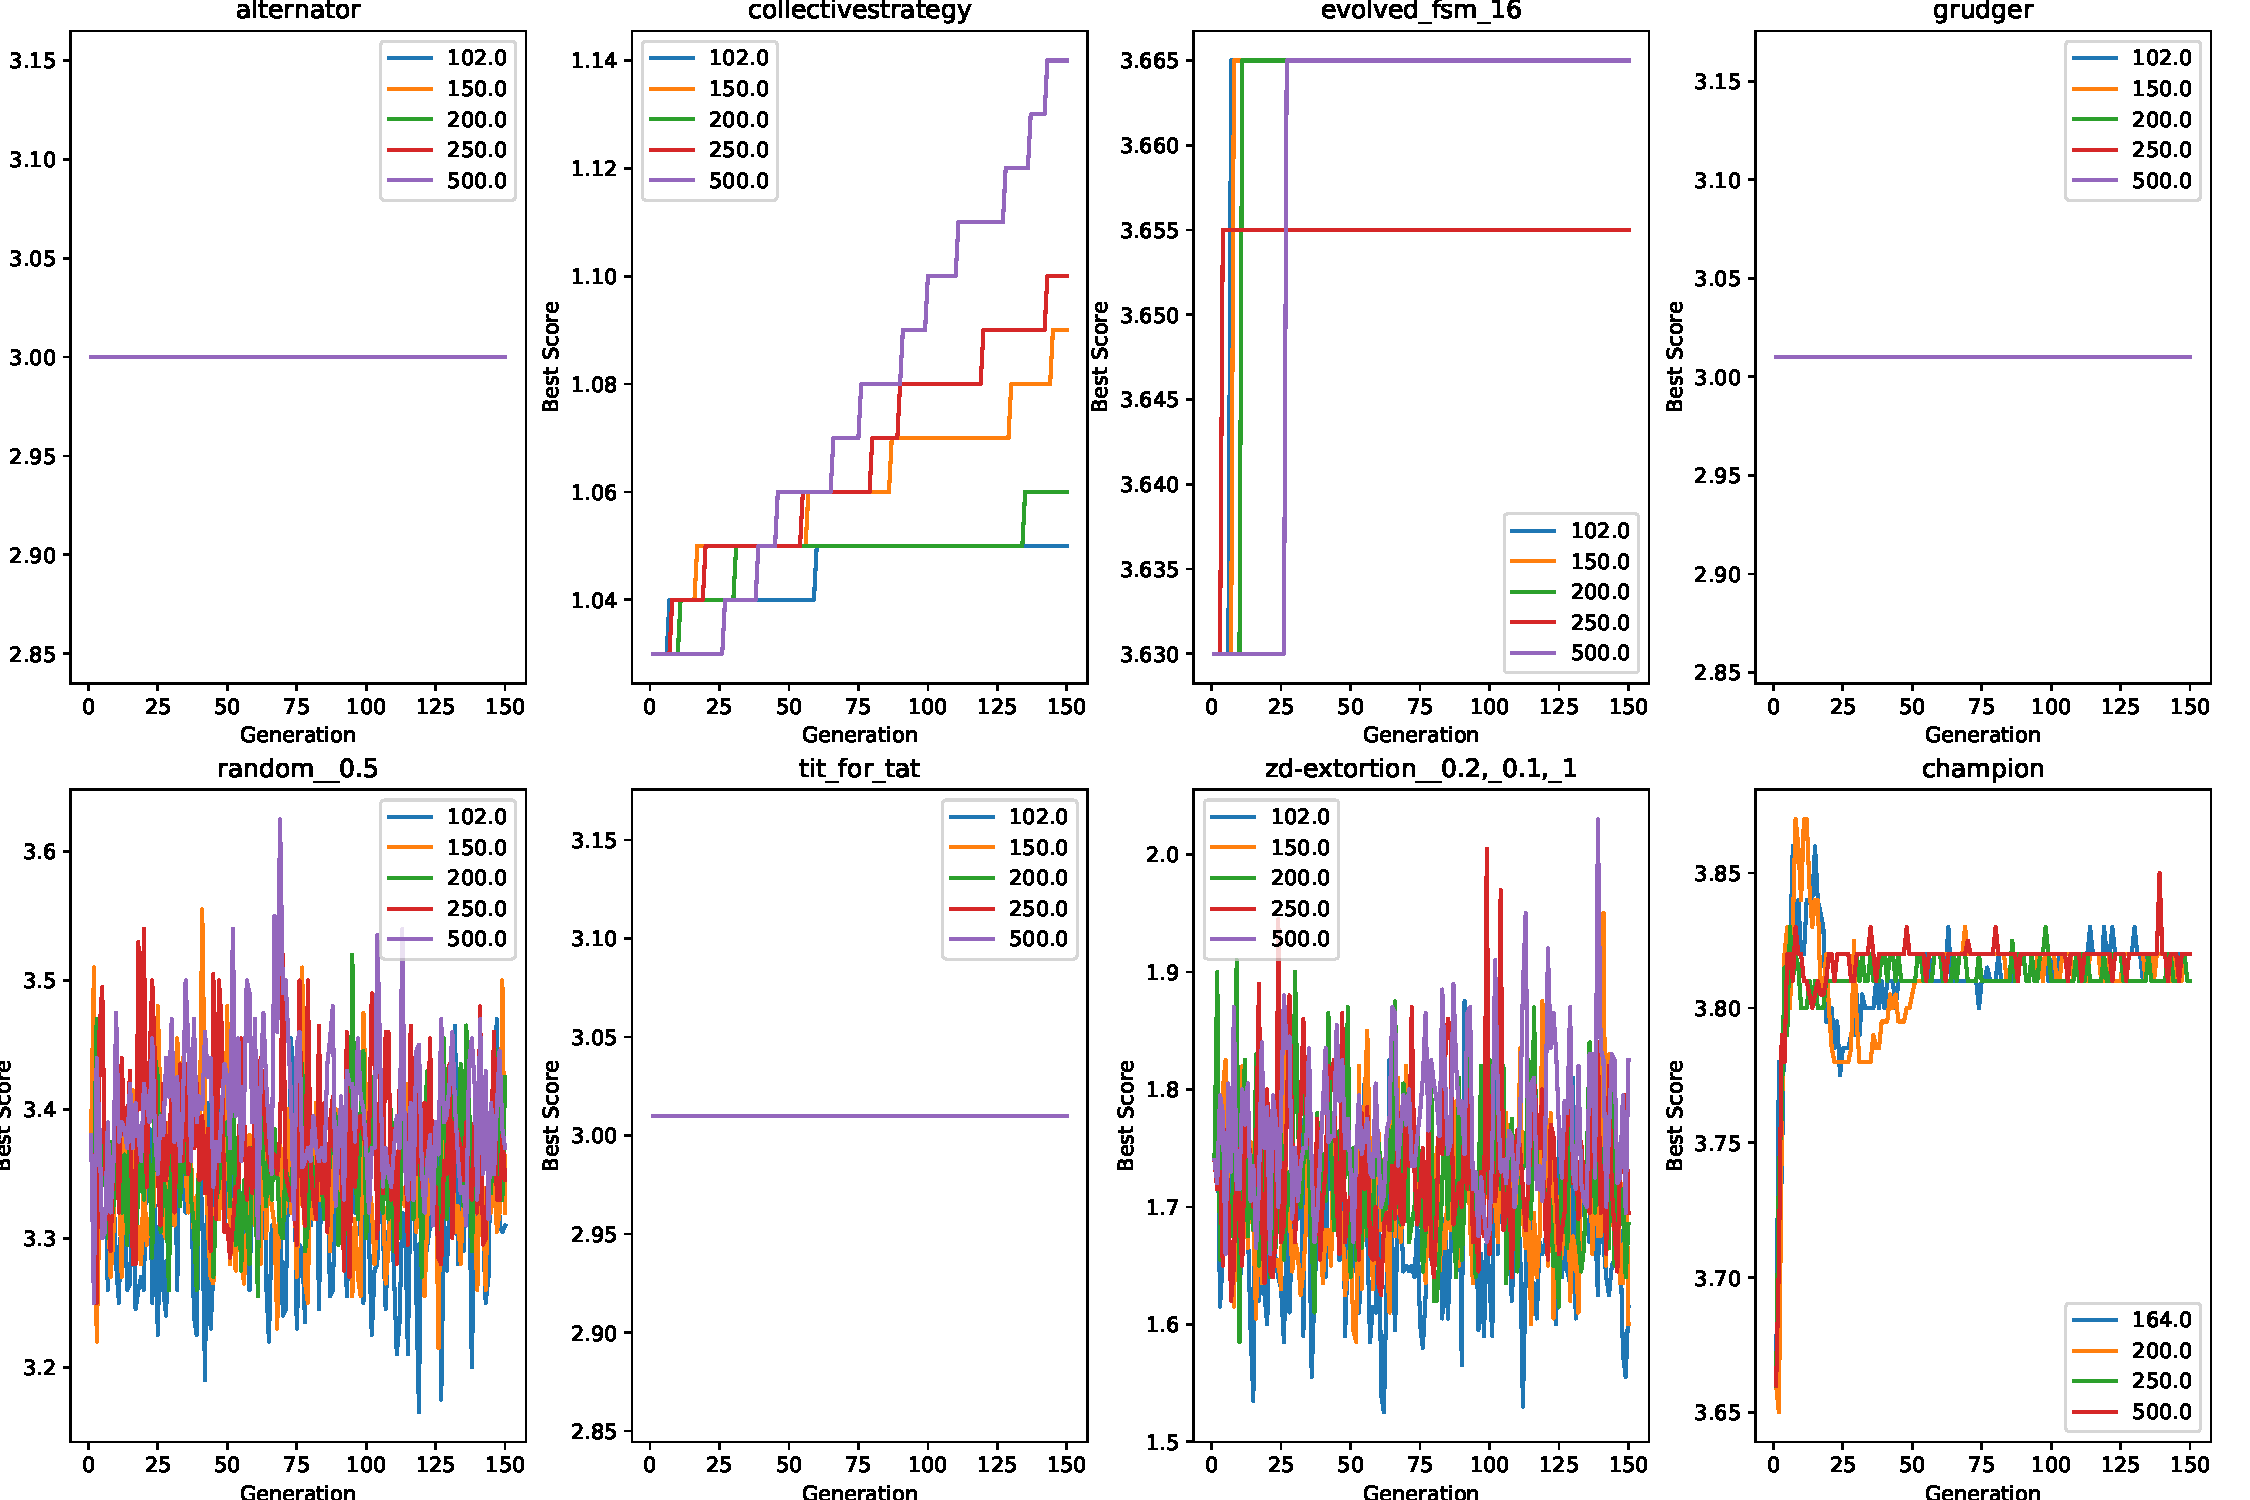
\includegraphics[width=0.8\textwidth, keepaspectratio, center]{./img/plots/NEW_INIT_POP_bs_v_gen_all_old.pdf}
    \caption{Best Score vs generations for pre-set initial populations on top of random sequences}\label{fig:NEW-INIT-POP-bs-v-gen-all}
\end{figure}

Figure~\ref{fig:NEW-INIT-POP-bs-v-gen-all} appears to have a better results for Collective Strategy with an initial set population for the algorithm.
Of the results that are not showing optimal solutions we can observe that the algorithm has score plateaus for all but Random, Collective Strategy, ZD Extort and Champion.
This is probably due to 2 different reasons:

\textbf{Random \& Stochastic Opponents}: This strategy should being beaten with a totality of D, the algorithm has in fact converged to almost this totality, but still has intermittent Cs.
The reason for this is the scoring grade `score per turn' will reflect on the number of intermittent Cs in the Random players sequence.
More Ds in the Random sequence will allow the solutions defections to score less.
This leads to a solution sequence containing some random Cs not because they score better in some turns, but because these tests not a fair trial.
The two sequences play against different Random opponents generation to generation without then being seeded.

\textbf{Collective Strategy}: This strategy is a combination of a handshake and the Grudger strategy.
If we look into the solution it would be seen to have found the handshake but then arrives on the Grudger effect later in the game.
After this encounter the same problem as we had before, with grudger, the algorithms limits the damage by splitting solutions into Cs then Ds.
Solving the collective strategy (and handshakes in general) may be simple;
we just put in all the possible n move handshakes followed by totalities and then set to work on the 2nd part of the sequence.
(*This means we increase our initial population from 102 members to 164)

It is clear that having a larger population is good from the old analysis, but the initial population still has to be tweaked to improve its scores against certain handshake opponents.
The Random and other stochastic opponents are a special cases that require more analysis to find the absolute optimal.
The new initial population, now of size 164, will include all combinations of C \& D of length 4, followed by finishing on all Cs or Ds as shown in the Totalities \& handshakes section of Snippet~\ref{code:initialPopulationCode}.
Further tests will also supplement this population with random members for \(|P| \in [164,200,250,500]\)

\begin{figure}[h]
    \inputminted{python}{code_snippets/initialPopulationCode.py}
    \caption{Initial Population Code}\label{code:initialPopulationCode}
\end{figure}

Figure~\ref{fig:NEW-INIT-POP-bs-v-gen-non-performers} shows the best score generation to generation for each population size, this time for the previous strategies where an optimal solution was not found.
After adding the extra members of the initial population we can see that now the handshake strategy (such as Collective Strategy) are solved much sooner.
Also shown is the Random and ZD extort players, these are examples of Stochastic players which are still not finding optimal solutions due to the observation of seeding stochastic opponents.
These classes of opponent are examined further in Section~\ref{sec:stochasticOpponents}.

\begin{figure}[h]
    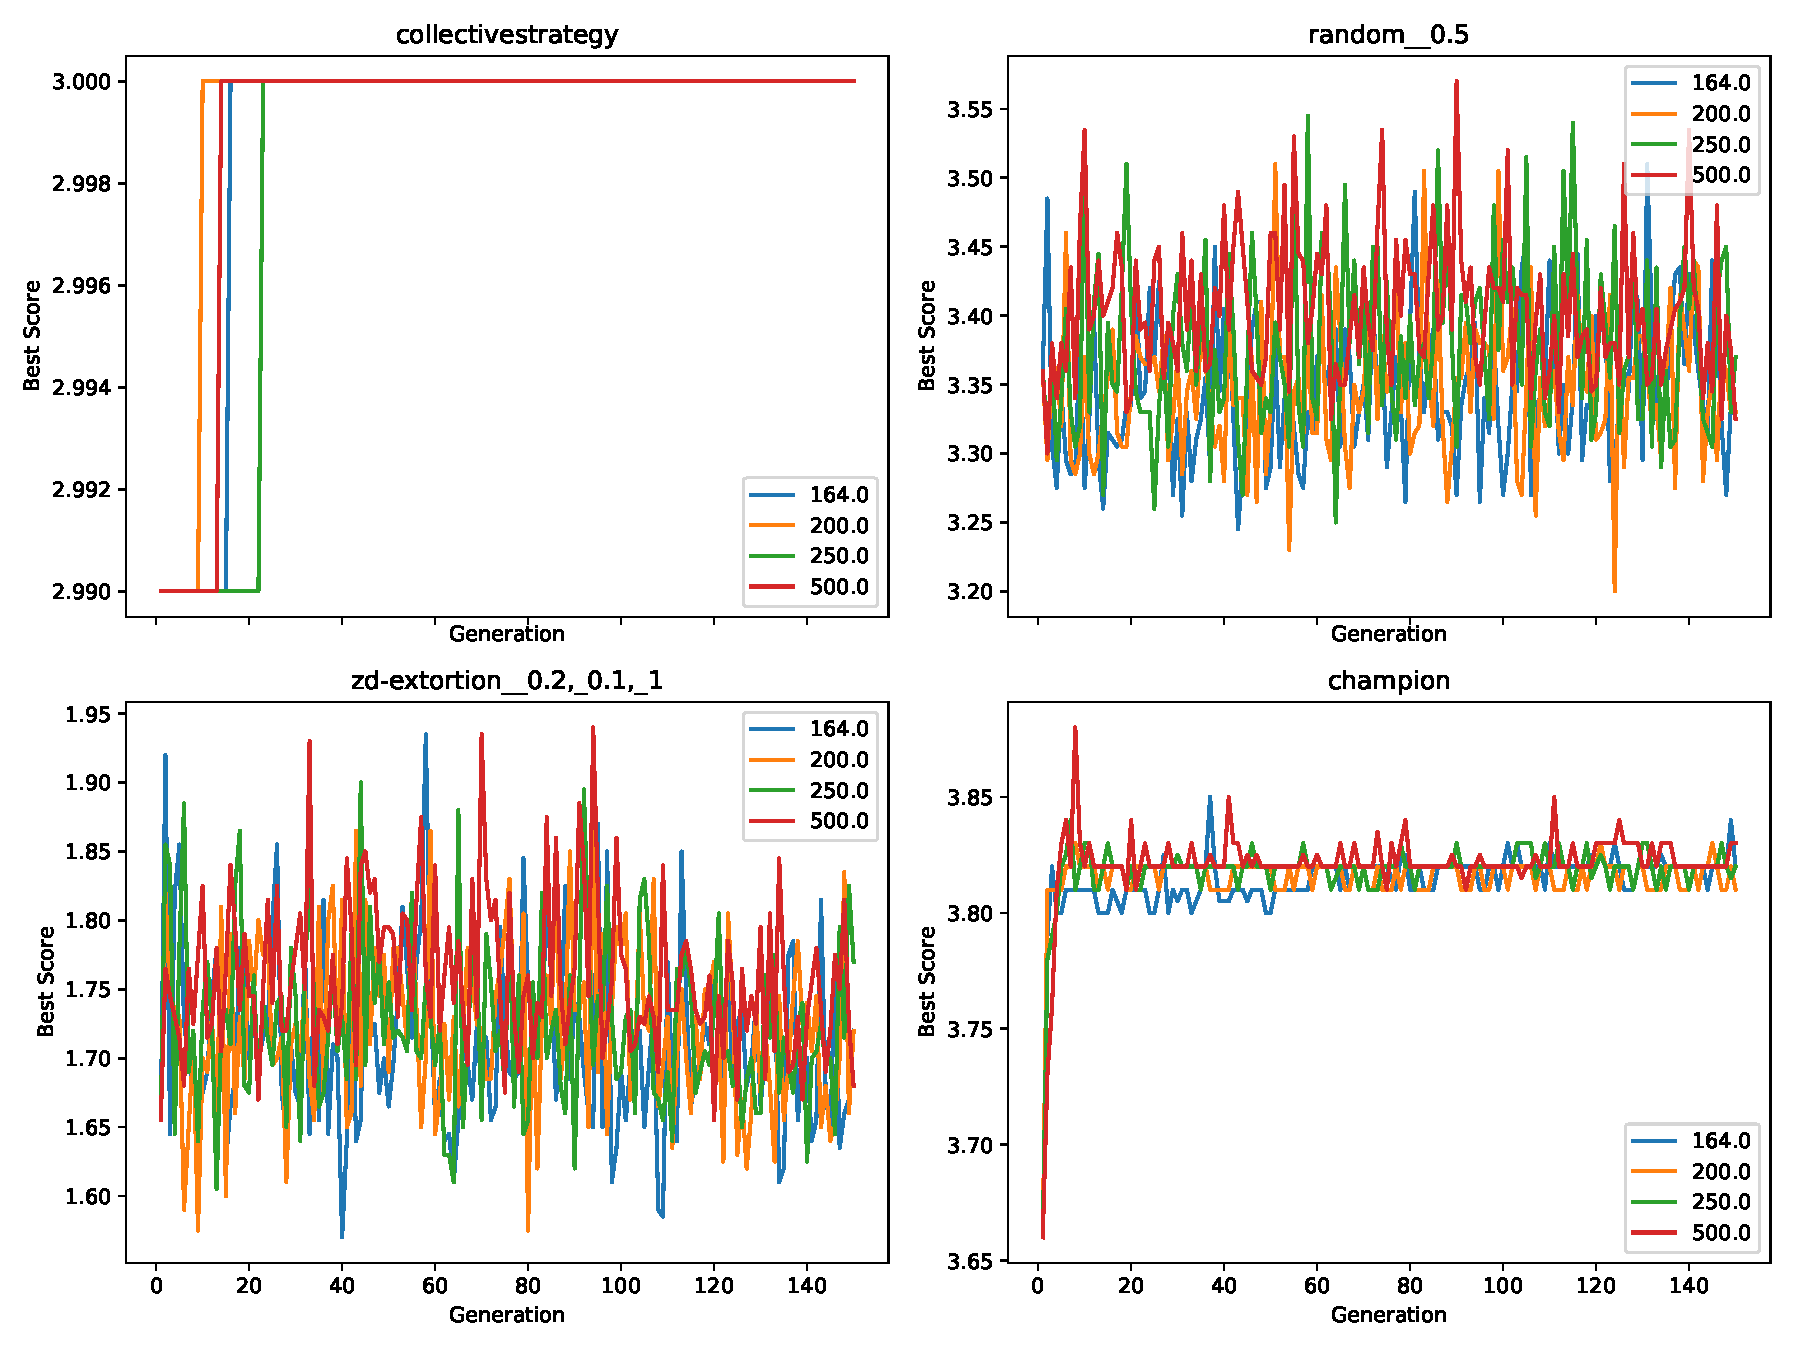
\includegraphics[width=0.8\textwidth, keepaspectratio, center]{./img/plots/NEW_INIT_POP_bs_v_gen_non_performers.pdf}
    \caption{\textbf{New Population:} Non optimal sequence players after changing initial population}\label{fig:NEW-INIT-POP-bs-v-gen-non-performers}
\end{figure}

It is clear the change of initial population is beneficial.
The actual parameter we will use in the full analysis will be given consideration in Section~\ref{sec:conclusionOfApproach}, but the initial population will stay as an effective starting point for the GA.

\subsection{Generation Length, Mutation Potency \& Mutation Frequency Analysis After Change of Initial Population}\label{subsec:starting_pop_analysis}
Figure~\ref{fig:NEW-GEN-bs-v-gen-all} shows how the best score is affected while changing the number of generations the algorithm will run to \(G \in [50,150,250,350,450,500] \).
This figure is also displaying with a population size of \(|P|=200\), 164 of which are pre defined.
It shows no real improvement from increasing the generations, the actual parameter we will use in the full analysis will be given consideration based off conclusions made in Section~\ref{sec:generationlengthanalysis}.

\begin{figure}[h]
    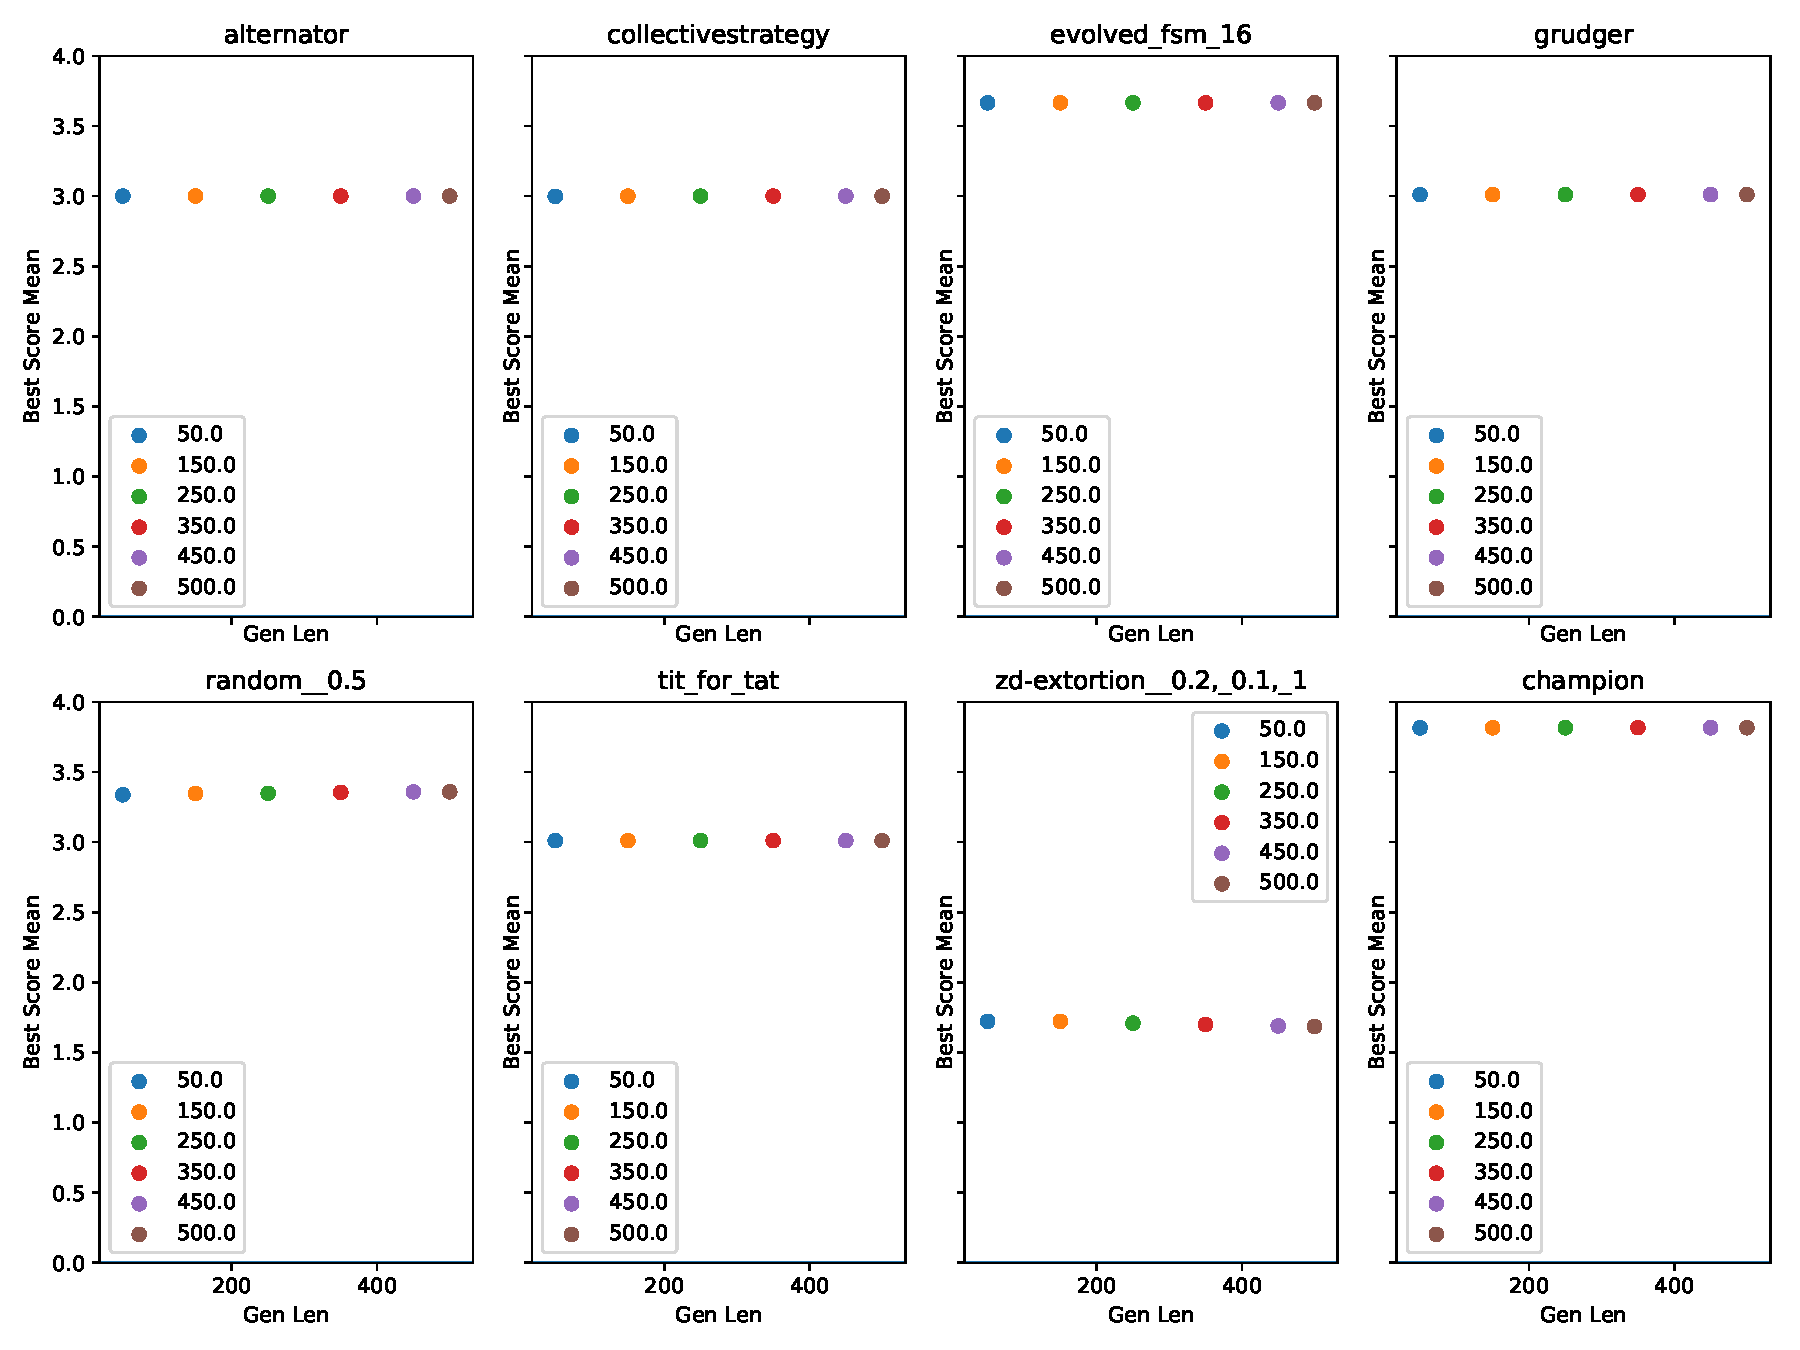
\includegraphics[width=0.8\textwidth, keepaspectratio, center]{./img/plots/NEW_GEN_bs_v_gen_all.pdf}
    \caption{\textbf{New Population:} Generation Length analysis for best score mean against generation length.}\label{fig:NEW-GEN-bs-v-gen-all}
\end{figure}

Figure~\ref{fig:NEW-MUT-POT-bs-v-gen-all} shows the best score generation to generation while changing the mutation potency.
\(M_p \in [1,2,3,5,10,15,20] \) was used whilst also running with a population size of \(|P|=200\).
The figure shows no real improvement from increasing this variable of the algorithm.
The actual parameter we will use in the full analysis will be given consideration based off conclusions made in Section~\ref{subsec:changingMutationPotency}.

\begin{figure}[h]
    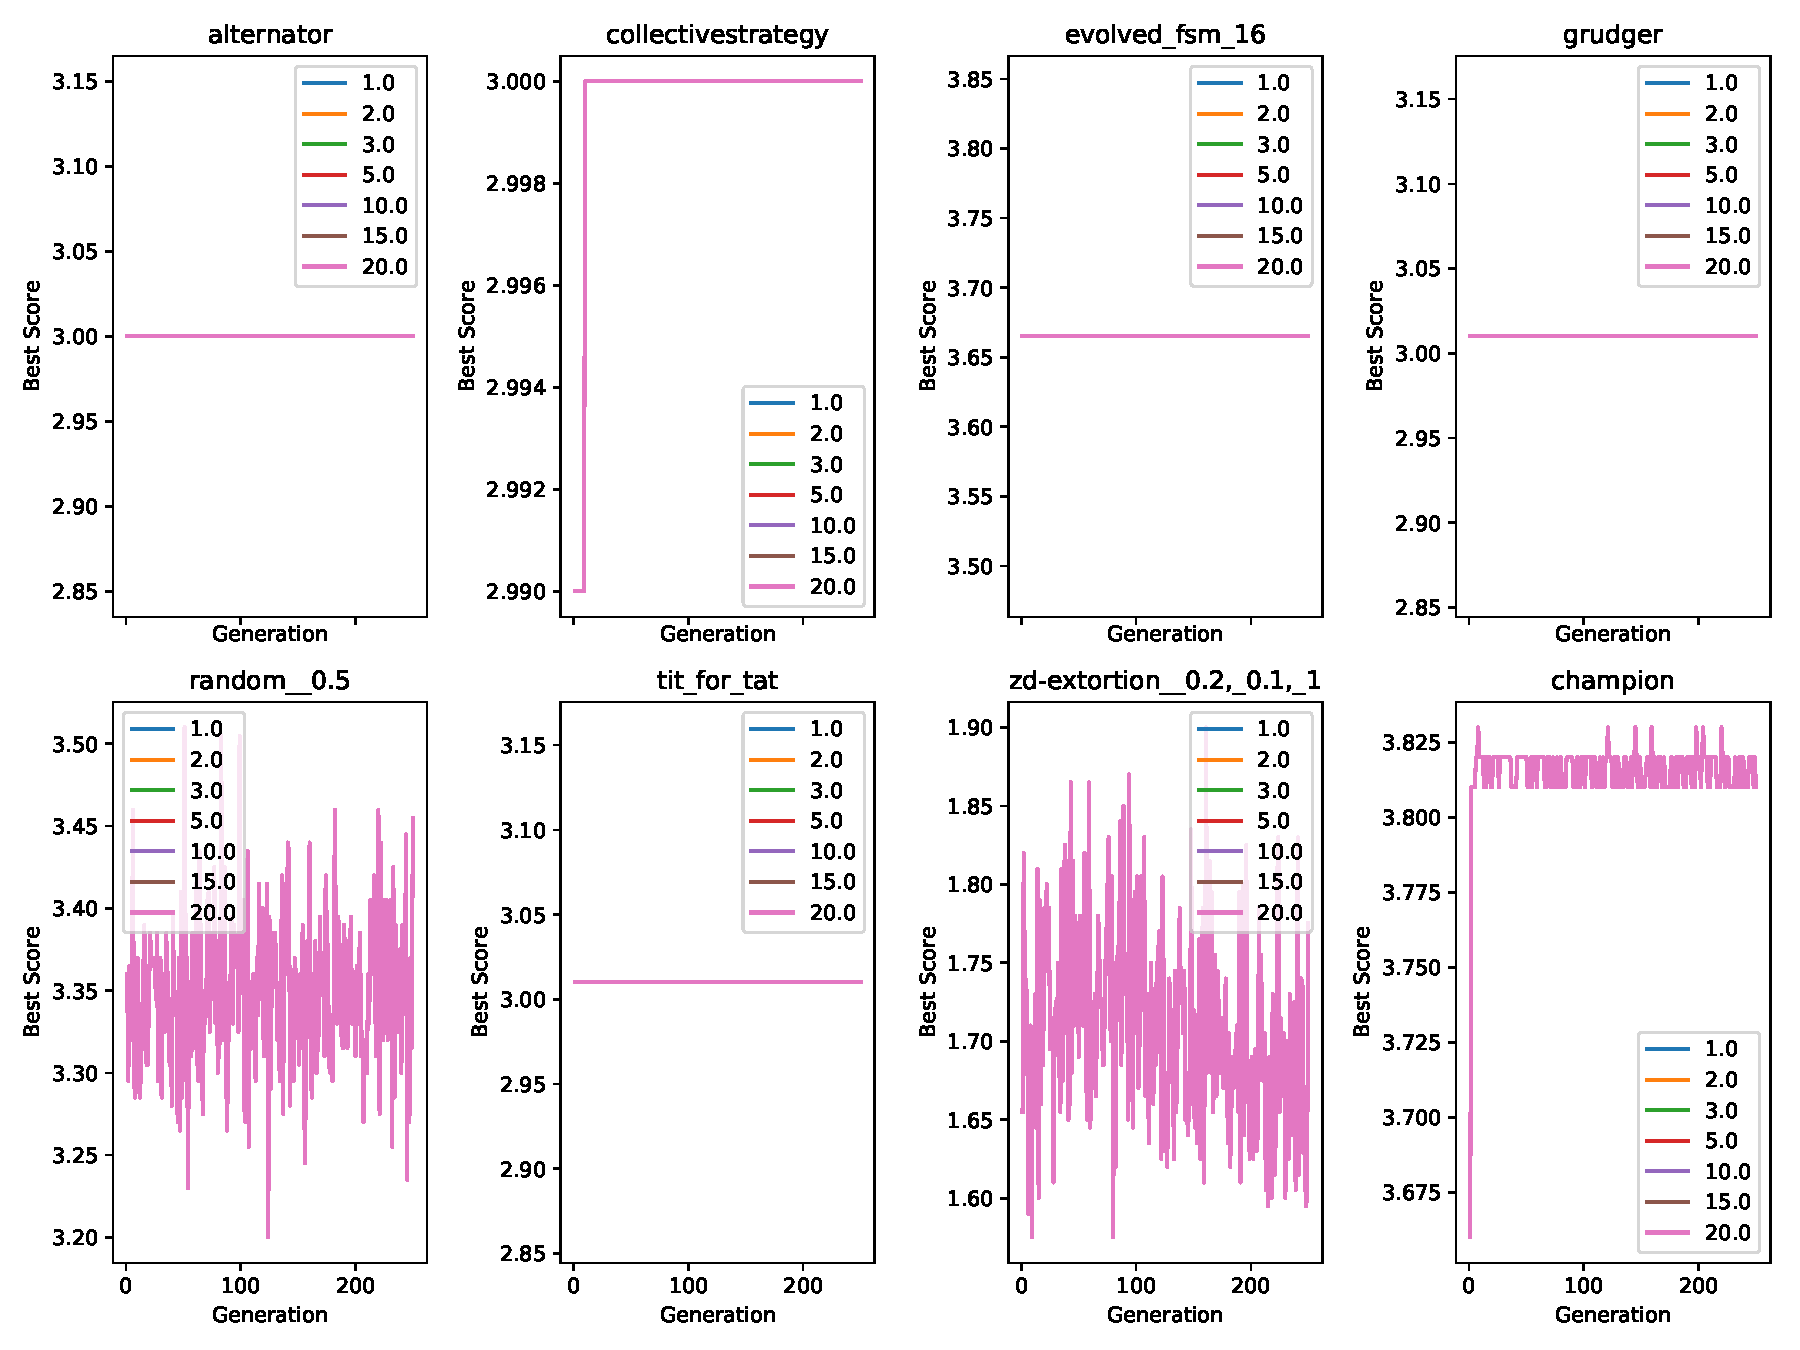
\includegraphics[width=0.8\textwidth, keepaspectratio, center]{./img/plots/NEW_MUT_POT_bs_v_gen_all.pdf}
    \caption{\textbf{New Population:} Best score against generation for different mutation potency levels}\label{fig:NEW-MUT-POT-bs-v-gen-all}
\end{figure}


Figure~\ref{fig:NEW-MUT-FREQ-bs-gen-all} shows the best score generation to generation while changing the mutation frequency.
\(M_f \in [0.1,0.15,0.2,0.25] \) was used whilst also running with a population size of \(|P|=200\).
The figure shows no real improvement from increasing this variable of the algorithm.
The actual parameter we will use in the full analysis will be given consideration based off conclusions made in Section~\ref{subsec:changingMutationFrequency}.

\begin{figure}[h]
    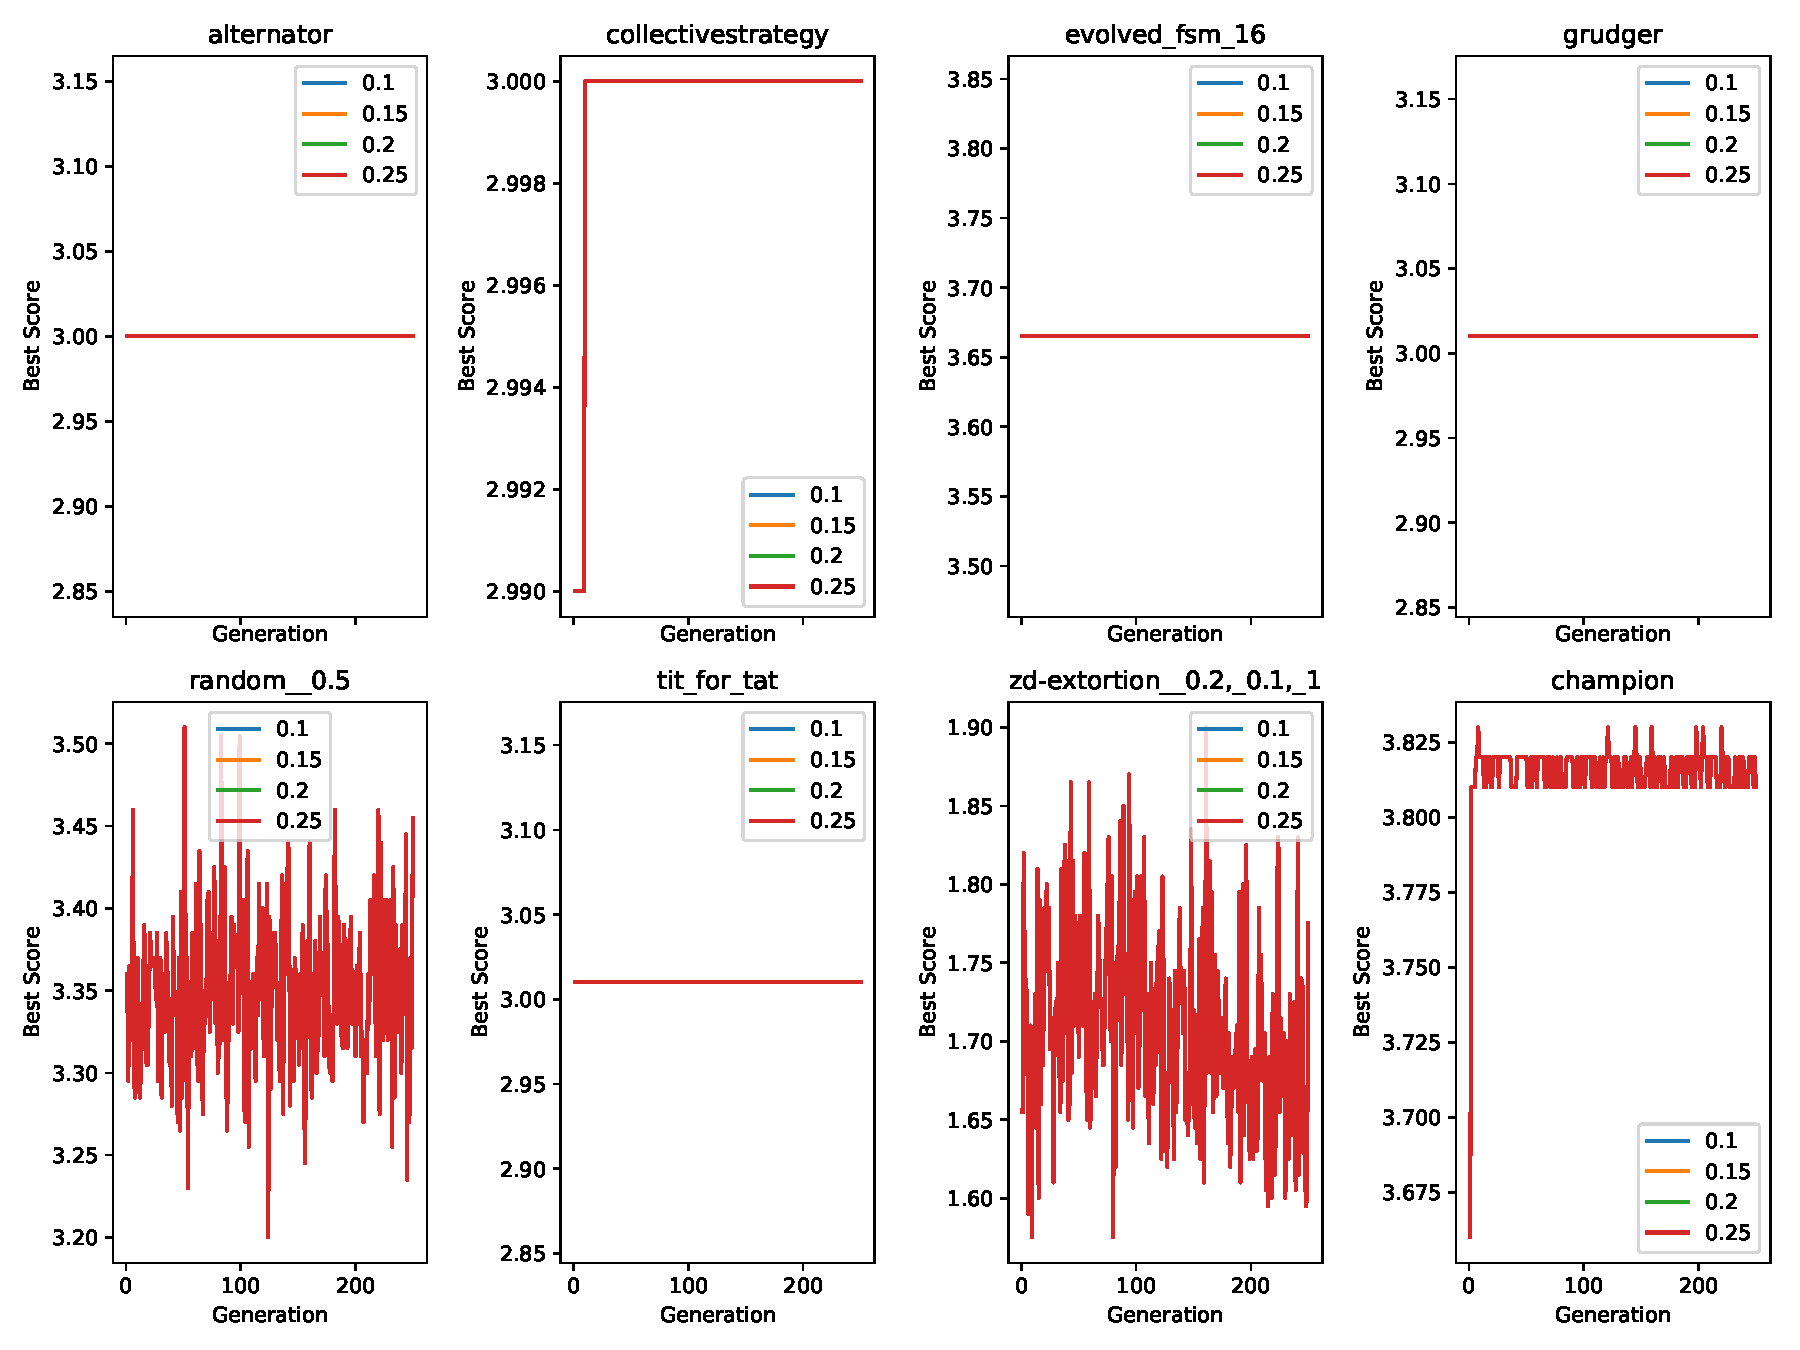
\includegraphics[width=0.8\textwidth, keepaspectratio, center]{./img/plots/NEW_MUT_FREQ_bs_v_gen_all.pdf}
    \caption{\textbf{New Population:} Best score against generation for different mutation frequencies}\label{fig:NEW-MUT-FREQ-bs-gen-all}
\end{figure}

\subsubsection{Discussion}\label{subsubsec:discussion}
The approach of adding a predefined set of members to the population before running the algorithm was incredibly successful.
Most opponents have solution sequence equal to or very close to members in the starting population.
This result will mean that when calculating the solution sequence for the main population the predefined set, generated by Snippet~\ref{code:initialPopulationCode}, will be used to shorten analysis times.

Random, ZDExtort and Champion are still being shown that the algorithm is not finding the optimal solution for these opponents.
This is due to the fact these player belong to the class of stochastic opponents.
Section~\ref{sec:stochasticOpponents} will look into these in more detail, putting forward a possible approach to simplify finding of a solution sequence for these opponents.

\section{Stochastic Opponents}\label{sec:stochasticOpponents}
Stochastic opponents create a problem with respect to continuity of testing.
The programming of the algorithm we are using generates a new opponent for every member every generation we run.
This, essentially, leads to the algorithm playing a new version of the opponent every time, leaving very little opportunity to identify features of stochastic opponents which can be exploited.

The concept of a stochastic opponent can be somewhat `overridden' by seeding the pseudo random number generator that creates the parameters that define what moves the strategy will take.
Currently the only way of doing this is by seeing the whole Axelrod library upon initialising the opponent instance.
Snippet~\ref{code:wrappingFunction} shows the code for wrapping any given opponent with the global seed command.

\begin{figure}[h]
    \inputminted{python}{code_snippets/classWrappingFunction.py}
    \caption{A function for wrapping a player with a global seed function call}\label{code:wrappingFunction}
\end{figure}

When calculating the solution sequence for all of the opponents we will do so with seeded versions of the stochastic opponents.
The parameters for stochastic opponents will be the default set by the creators and new instances will be made with the seed that is set for algorithm as a whole.
The means we will be playing the same `version' of a stochastic opponent over and over, removing the layer of abstraction in its strategy.

\section{Conclusion of approach}\label{sec:conclusionOfApproach}
Each section of testing allowed the algorithm to become more specialised in solving the given task.
The list at the end of this section shows which parameters we have chosen for the final analysis.

After constructing the final analysis factory and running some environment checks we made the following changes to the code for ease of use:
\begin{itemize}
    \item Number of generations changed: $300\rightarrow600$.
    \item Crossover algorithm, shown in Figure~\ref{fig:newCrossover}, was reverted to code given in Figure ~\ref{fig:oldCrossover}
\end{itemize}

These changes resulted in a streamlined piece of code we were able to run on the Cardiff University Mathematics department big compute machine.
Reflecting on the execution and deployment of the code shows that we could have improved the analysis of short run time strategies against longer run time strategies and the reproducibility of the batch processing within the Axelrod Dojo Module.
As far as each individuals analysis goes, I feel like the approach of adding predetermined sequences to an initial population was a huge improvement in compute time and overall predictions of best sequences. 

The algorithm parameters described in section~\ref{subsec:geneticAlgorithms} have the following parameters before running the final analysis:
\begin{itemize}
    \item Initial Population, $P$, of 164 pre generated members + 86 random members for a total of 250.
    \item Generation length, $G$, of 600.
    \item Mutation Potency, $M_p$, of 1.
    \item Mutation Frequency, $M_f$, of 0.1.
    \item Bottleneck, $b=P/4$.
    \item Crossover method as that shown in Snippet~\ref{fig:oldCrossover}.
    \item Mutation method as that shown in Snippet~\ref{apcode:mutateFromDojo}
    \item Each opponent is wrapped in the seed wrapper shown in Snippet~\ref{code:wrappingFunction}, stochastic opponents will be run 10 times each with different seeds.
\end{itemize}